\documentclass[12pt]{article}
\usepackage[utf8]{inputenc}
\usepackage[margin=0.6in, top=0.8in, bottom=1in]{geometry}
\setlength\columnsep{1cm}
\usepackage{amsmath}
\usepackage{amssymb}
\usepackage{float}
\usepackage{comment}
\usepackage{amsthm}
\geometry{a4paper}
\usepackage{graphicx}
\usepackage{booktabs}
\usepackage{array}
\usepackage{paralist}
\usepackage{verbatim}
\usepackage{multirow}
\usepackage{multicol}
\usepackage{rotating}
\usepackage{fancyhdr}
\usepackage{hyperref}
\usepackage{cleveref}
\pagestyle{fancy}
\renewcommand{\headrulewidth}{0pt}
\lhead{}\chead{}\rhead{}
\lfoot{}\cfoot{\thepage}\rfoot{}
\usepackage{sectsty}
\allsectionsfont{\sffamily\mdseries\upshape}
\usepackage{fancyvrb}
\usepackage{bm}
\usepackage{bbm}
\usepackage{subfigure}
\usepackage{mathtools}
\usepackage[mathscr]{eucal}
\usepackage[ruled, lined, linesnumbered, commentsnumbered, longend]{algorithm2e}
\usepackage{multirow}
\usepackage[table,xcdraw]{xcolor}

\theoremstyle{definition}
\newtheorem{definition}{Definition}[section]
\theoremstyle{definition}
\newtheorem{theorem}{Theorem}[section]
\theoremstyle{lemma}
\newtheorem{lemma}{Lemma}[section]
\theoremstyle{remark}
\newtheorem{remark}{Remark}[section]
\theoremstyle{definition}
\newtheorem{proposition}{Proposition}[section]


\newcommand{\indep}{\perp \!\!\! \perp}

%%set of code frame
\usepackage{listings}
\usepackage{xcolor}
\definecolor{codegreen}{rgb}{0,0.6,0}
\definecolor{codegray}{rgb}{0.5,0.5,0.5}
\definecolor{codepurple}{rgb}{0.58,0,0.82}
\definecolor{backcolour}{rgb}{0.95,0.95,0.92}

\lstdefinestyle{mystyle}{
    backgroundcolor=\color{backcolour},
    commentstyle=\color{codegreen},
    keywordstyle=\color{blue},
    numberstyle=\tiny\color{codegray},
    stringstyle=\color{codepurple},
    basicstyle=\ttfamily\footnotesize,
    breakatwhitespace=false,
    breaklines=true,
    captionpos=b,
    keepspaces=true,
    showspaces=false,
    showstringspaces=false,
}
\newcommand\numberthis{\addtocounter{equation}{1}\tag{\theequation}}


\lstset{style=mystyle}

\usepackage{xcolor}
\usepackage[numbers]{natbib}

% cleveref needs the name for algorithm2e's float type (algocf)
\crefname{algocf}{Algorithm}{Algorithms}
\Crefname{algocf}{Algorithm}{Algorithms}


\title{Annual Progress Monitor(APM) Report}
\author{QI CHEN}
\date{Feb 2026}

\begin{document}
\maketitle

\setcounter{section}{-1}
\section{Project Overview, Timeline, and Thesis Outline}\label{sec:overview}

\subsection{Overview}
The thesis develops statistical methods for reconstructing \emph{admixture
graphs} --- demographic histories in which populations not only split but also
mix --- from genetic data, and applies them to human population history.

The core methodological problem is that the two most informative kinds of genetic
signal speak to different time depths. \emph{Identity-by-descent (IBD) segments}
are long stretches of genome co-inherited from a recent common ancestor; their
length distribution is sharply informative about \emph{recent} demographic events
but is erased by recombination at greater depths. \emph{Single-nucleotide
polymorphism (SNP) allele frequencies}, summarized through their cross-population
covariance ($f$-statistics), carry the complementary signal of \emph{ancient}
shared drift. The central idea of the thesis is to combine the two in a single
\emph{composite likelihood} for the admixture graph: an analytic expectation of
IBD sharing as a function of the graph (derived here via a matrix recursion over
epochs), a TreeMix-style model for the SNP covariance, and a shared parameter
vector (event times, admixture fractions, effective sizes) fitted by Bayesian
variational inference. Candidate graph topologies are compared as competing
models through their evidence (ELBO), turning topology choice into a question of
statistical model selection.

The work proceeds in three stages of increasing ambition. The first builds and
validates the composite-likelihood framework for a \emph{given} topology. The
second tackles the combinatorially large space of admixture graphs directly: an
efficient graph search (using TreeMix, or an alternative, to initialize the
placement of admixture events) together with topology selection cast as
statistical hypothesis testing and as the combination of subgraphs inferred on
subsets of populations. The third turns to \emph{application}: integrating the
genetic admixture-graph inferences with \emph{linguistic} data, relating the
history of populations to the history of their languages.

\subsection{PhD Timeline}
\Cref{tab:timeline} summarizes the planned timeline and the current status of each
phase. The first phase --- the methodological framework that is the subject of
\crefrange{sec:ibd}{sec:simstudy} of this report --- is complete and validated on
simulated data; the graph-search phase is under way; the linguistic-application
phase is planned for the remainder of the PhD.

\begin{table}[!htbp]
\centering
\renewcommand{\arraystretch}{1.3}
\begin{tabular}{p{3.0cm} p{8.5cm} p{1.6cm} l}
\toprule
\textbf{Period} & \textbf{Activity / deliverable} & \textbf{Thesis part} & \textbf{Status} \\
\midrule
Jun--Jul 2025 &
Analysis of real data and write-up of the first paper: the composite IBD\,+\,SNP
inference framework for a given admixture graph (no efficient graph search). &
Part I &
\textcolor{codegreen}{\textbf{Completed}} \\
Aug--Nov 2025 &
A new (or extended) dataset with more populations; optimization via graph search
--- TreeMix (or another method) as an initialization for admixture placement,
followed by topology selection as statistical testing / combination of subgraphs
on sub-populations. &
Part II &
\textcolor{orange}{\textbf{In progress}} \\
Late 2025 -- end of PhD &
Integration with linguistic data; broader applications relating genetic and
language history. &
Part III &
\textcolor{red}{\textbf{Planned}} \\
\bottomrule
\end{tabular}
\caption{PhD timeline and status of each phase.}\label{tab:timeline}
\end{table}

\subsection{Thesis Outline}
The thesis is organized into three parts, mirroring the timeline. Below, each
part is broken down into its components with the current status indicated as
\textcolor{codegreen}{\textbf{[done]}},
\textcolor{orange}{\textbf{[in progress]}}, or
\textcolor{red}{\textbf{[planned]}}.

\paragraph{Part I --- A composite-likelihood framework for admixture-graph
inference from IBD and SNP data, for a given topology.}
This part corresponds to \crefrange{sec:ibd}{sec:simstudy} of the present report.
\begin{compactitem}
  \item \textcolor{codegreen}{\textbf{[done]}} Analytic expectation of IBD
  segment sharing under an admixture graph: the per-epoch contribution
  $f(t_1,t_2,N,u,v)$ and its accumulation by a matrix recursion over an arbitrary
  topology (\cref{sec:algorithm}).
  \item \textcolor{codegreen}{\textbf{[done]}} Zero-observation (Poisson)
  adjustment for empty length bins (\cref{sec:zero}), and block-bootstrap with a
  delete-one-haplotype jackknife for the IBD variance (\cref{sec:estimation}).
  \item \textcolor{codegreen}{\textbf{[done]}} SNP allele-frequency covariance
  model (Brownian drift + linear admixture, double-centered TreeMix estimator)
  (\cref{sec:snp}).
  \item \textcolor{codegreen}{\textbf{[done]}} Composite IBD\,+\,SNP likelihood,
  Bayesian inference via Pathfinder variational inference, and topology selection
  through the ELBO (\cref{sec:framework}).
  \item \textcolor{codegreen}{\textbf{[done]}} Simulation validation: parameter
  recovery under uniform and varying effective sizes; the recent-vs-ancient
  division of labor between IBD and SNP; Pathfinder-vs-HMC bias and efficiency;
  and robustness to estimated (Hap-IBD) rather than true segments
  (\cref{sec:simstudy}).
  \item \textcolor{orange}{\textbf{[in progress]}} Application to a real dataset
  and write-up as the first paper.
\end{compactitem}

\paragraph{Part II --- Scaling to many populations: efficient admixture-graph
search and topology selection as statistical testing.}
\begin{compactitem}
  \item \textcolor{orange}{\textbf{[in progress]}} Assembling a larger
  multi-population dataset (a new dataset, or the existing one extended with more
  populations).
  
  \item \textcolor{codegreen}{\textbf{[done]}} Topology selection framed as
  statistical hypothesis testing (is an extra admixture edge supported by the
  data?), building on the ELBO-based model comparison of Part~I.
  \item \textcolor{red}{\textbf{[in progress]}} An efficient search over the space of
  admixture graphs, using TreeMix (or an alternative) to initialize the number
  and placement of admixture events rather than enumerating topologies blindly.
  \item \textcolor{red}{\textbf{[in progress]}} Combining subgraphs inferred on
  subsets of populations into a coherent global admixture graph, to keep the
  search tractable as the number of populations grows.
  \item \textcolor{red}{\textbf{[planned]}} Validation on simulations and
  application; write-up as the second paper.
\end{compactitem}

\paragraph{Part III --- Integrating genetic and linguistic data.}
\begin{compactitem}
  \item \textcolor{red}{\textbf{[planned]}} Curation of linguistic data
  (phylogenies and/or contact/borrowing information) aligned to the genetic
  populations.
  \item \textcolor{red}{\textbf{[planned]}} Joint or comparative analysis of the
  inferred genetic admixture graphs against language history, testing where
  genetic and linguistic signals of contact agree or diverge.
  \item \textcolor{red}{\textbf{[planned]}} Case-study applications and final
  write-up.
\end{compactitem}

\section{Inference via Identity by Descent(IBD segment)}\label{sec:ibd}
We will use the average fraction of the genome shared through Identity by Descent(IBD) segments of length between $u$ centiMorgans and  $v$ centiMorgans. Here, $u$ and $v$ are given. The explicit formula for the expectation of the above statistics is as follows. \begin{equation}\label{eq:expectation_fraction}
    \mathbb{E}_{[u,v]}[f|\theta] =\frac{1}{|I|}\sum_{i\in I}\mathbb{E}[\mathbbm{1}\{u\leq l_i\leq v\}|\theta]= \frac{1}{|I|}\sum_{i\in I}p(u\leq l_i\leq v|
\theta) = p(u\leq L\leq v|\theta)
\end{equation}
We treat the continuous genome as a discrete set $I$ of sites. $l_i$ is the length of the IBD segments containing site $i$. Thus, we are left to compute the probability that a site is contained in an IBD segment of length $l$, where $l$ is between $u$ and $v$.

If we are interested in the probability that IBD segments lie in the length range $R=[u,v]$ then \begin{align*}
    p(L\in R|\theta) &= \int_{t_1=0}^{t_2=\infty}\int_u^v p(L=l|g)p(g|\theta) dl dg\\
    &= \int_{t_1=0}^{t_2=\infty} p(g|\theta)\int_u^v (\frac{g}{50})^2l\exp(-\frac{g}{50}l)dl dg\\
    &= \int_{t_1=0}^{t_2=\infty} p(g|\theta) \left(\exp(-\frac{u}{50}g)(\frac{u}{50}g+1) - \exp(-\frac{v}{50}g)(\frac{v}{50}g+1)\right) dg
\end{align*}
Thus, modeling the distribution of coalescence in different epochs will give us an explicit formula for the expectation of total fraction of the genome. We choose the Wright-Fisher model for the probability of coalescing, that is, time follows a exponential distribution with rate as the effective population size.

Suppose that we are interested in the contribution between time $t_1$ and $t_2$ where the effective population size is fixed to $N$, then we will have the explicit formula:
\begin{align*}
   g(t_1, t_2, N, u, v) = &\int_{t_1}^{t_2} p(t|\theta) \left(\exp(-\frac{u}{50}t)(\frac{u}{50}t+1) - \exp(-\frac{v}{50}t)(\frac{v}{50}t+1)\right) dt\\
    &= s \times \int_{t_1}^{t_2} \frac{1}{N}\exp(-\frac{(t-t_1)}{N}) \left(\exp(-\frac{u}{50}t)(\frac{u}{50}t+1) - \exp(-\frac{v}{50}t)(\frac{v}{50}t+1)\right) \\
    &= s \exp(\frac{t_1}{N})\times \left(\frac{u}{50N}\left(\left[\frac{\exp(c_ut)(c_ut-1)}{c_u^2}\right]_{t=t_1}^{t=t_2}\right)  + \frac{1}{N}\left[\frac{\exp(c_ut)}{c_u}\right]_{t=t_1}^{t=t_2}\right)\\
    &\;\;- s \exp(\frac{t_1}{N})\times\left(\frac{v}{50N}\times\left(\left[\frac{\exp(c_vt)(c_vt-1)}{c_v^2}\right]_{t=t_1}^{t=t_2}\right) - \frac{1}{N}\left[\frac{\exp(c_vt)}{c_v}\right]_{t=t_1}^{t=t_2}\right)\\
    &= s \times f(t_1,t_2,N,u,v)\numberthis\label{eqn:linr|theta}
\end{align*}
where $c_u = -\left(\frac{1}{N}+\frac{u}{50}\right)$, $c_v = -\left(\frac{1}{N}+\frac{v}{50}\right)$ and $s$ represent a survival function that will be clear later. If we only consider one population, and we have the same population size throughout the time, then we can simply drop different epochs(since the term $\exp(\frac{t_1}{N})$ cancels out with $s$) and let $t_1$ be zero and $t_2$ be infinity. Working with a multi-population structure makes splitting time into different epochs inevitable.

\begin{figure}[!htbp]
    \centering
	    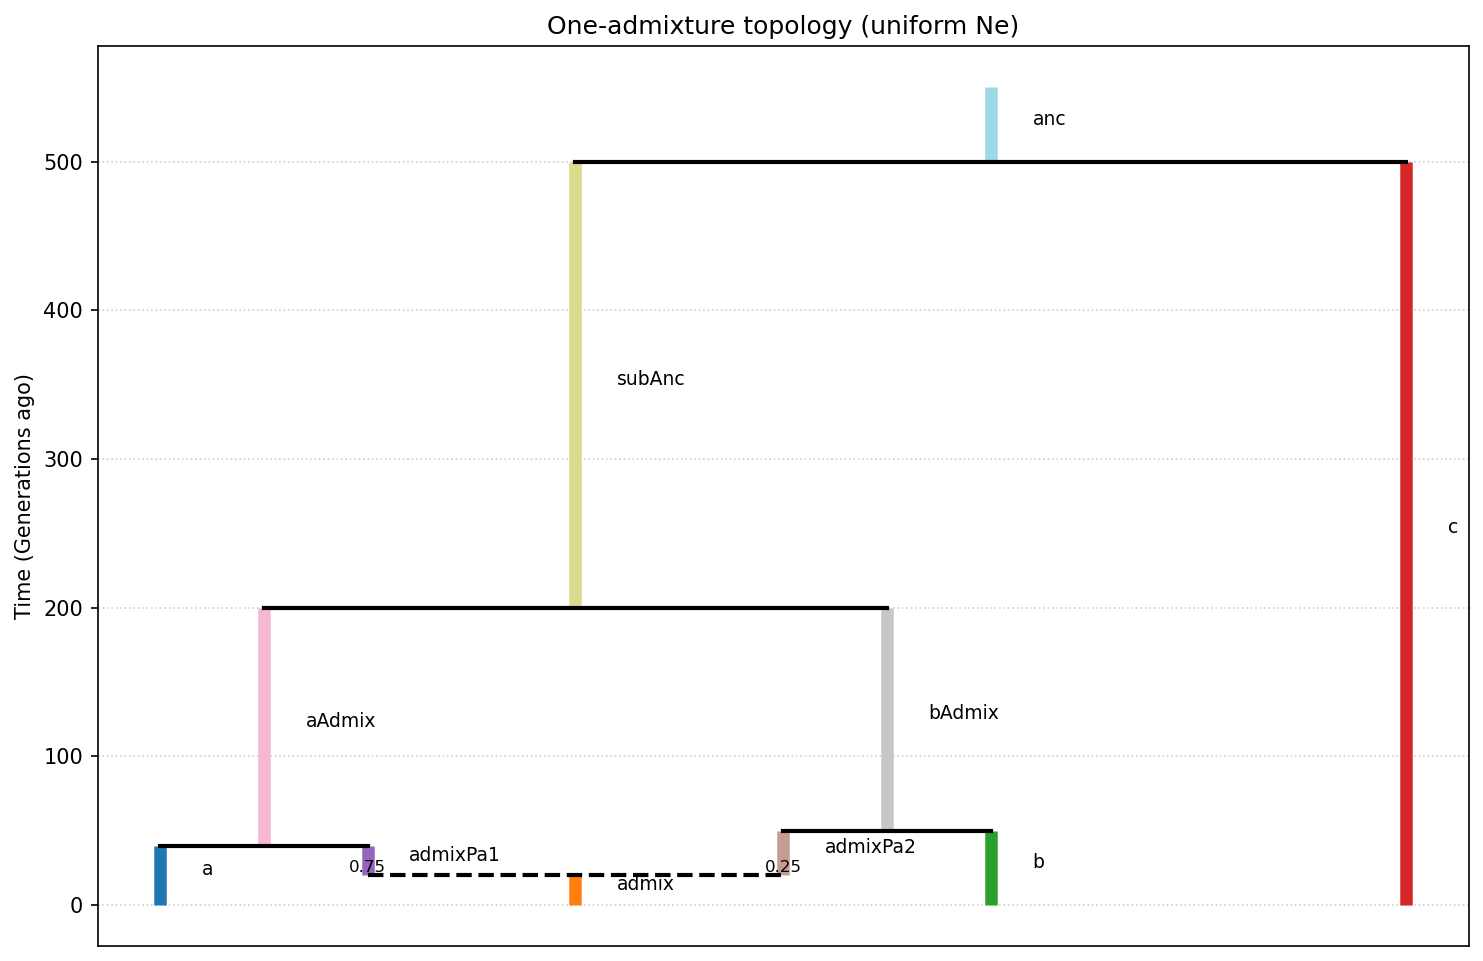
\includegraphics[width=15cm]{topology_example.png}
		\caption{Example of population history
		}\label{fig:topology_example}
	\end{figure}

\ref{fig:topology_example} shows an example of the demographic structures we will work with. The population 'admix' splits into two populations, 'admixPa1' and 'admixPa2' backward in time, and they then merge with 'a' and 'b' separately, then merge to form 'subanc' and finally everything leads to 'anc'. We define each epoch as a continuous time interval separated by different events. For example, in \ref{fig:topology_example} we have 6 epochs in total. We further assume that each event will generate a new population with its own population size, and population size is held constant for each population.

In order to model the probability distribution to the first coalescence time, we define the survival function \[S(N, t_a, t_b) = \exp\left(-\frac{t_b - t_a}{N}\right)\] as the total probability that two lineages in the same population of size $N$ do not coalesce between time $t_a$ and $t_b$.

As a working example, we derive the expectation of genome fraction shared through IBD segments between length $u$ and $v$ for population 'admix' and itself. Suppose that the admixture ratio is $\alpha$ to 'admixPa1' and thus $1-\alpha$ to 'admixPa2'. The first epoch will have contribution $f(0, t_1, N_{admix}, u, v)$, with survival probability $S(N_{admix}, 0, t_1)$ passed to the second epoch. The second epoch consists of the contribution from 'admixPa1' and the contribution from 'admixPa2'. The contribution is \[S(N_{admix},0,t_1)\times\left(\alpha^2 f(t_1,t_2, N_{admixPa1}, u, v) +(1-\alpha)^2 f(t_1, t_2, N_{admixPa2}, u, v)\right) \]

For the third epoch we will have \begin{align*}
&\alpha^2S(N_{admix}, 0, t_1)S(N_{admixPa1},t_1,t_2)f(t_2, t_3, N_{aAdmix}, u, v) \\ +&(1-\alpha)^2S(N_{admix}, 0, t_1)S(N_{admixPa2},t_1,t_2)f(t_2, t_3, N_{admixPa2}, u, v)
\end{align*}

For the fourth epoch, this will be \begin{align*}
&\alpha^2S(N_{admix}, 0, t_1)S(N_{admixPa1},t_1,t_2)S(N_{aAdmix}, t_2, t_3)f(t_3, t_4, N_{aAdmix}, u, v) \\ +&(1-\alpha)^2S(N_{admix}, 0, t_1)S(N_{admixPa2},t_1,t_2)S(N_{admixPa2}, t_2,t_3)f(t_3, t_4, N_{bAmix}, u, v)
\end{align*}

Now for the fifth epoch, since there are three tracks for lineages from 'admix' to 'subAnc', we have three separate contributions:\begin{align*}
&\alpha^2S(N_{admix}, 0, t_1)S(N_{admixPa1},t_1,t_2)S(N_{aAdmix}, t_2, t_3)S(N_{aAdmix}, t_3, t_4)f(t_4, t_5, N_{subAnc}, u, v) \\ +&(1-\alpha)^2S(N_{admix}, 0, t_1)S(N_{admixPa2},t_1,t_2)S(N_{admixPa2}, t_2,t_3)S(N_{bAdmix},t_3,t_4)f(t_4, t_5, N_{subAnc}, u, v)\\
+&2\alpha(1-\alpha)S(N_{admix}, 0, t_1)f(t_4, t_5, N_{subAnc}, u, v)
\end{align*}

And finally, for the last epoch to $\infty$ time, we have
\begin{align*}
&\alpha^2S(N_{admix}, 0, t_1)S(N_{admixPa1},t_1,t_2)S(N_{aAdmix}, t_2, t_3)S(N_{aAdmix}, t_3, t_4)S(N_{subAnc}t_4, t_5)f(t_5, \infty, N_{anc}, u, v) \\ +&(1-\alpha)^2S(N_{admix}, 0, t_1)S(N_{admixPa2},t_1,t_2)S(N_{admixPa2}, t_2,t_3)S(N_{bAdmix},t_3,t_4)S(N_{subAnc},t_4, t_5)f(t_5, \infty, N_{anc}, u, v)\\
+&2\alpha(1-\alpha)S(N_{admix}, 0, t_1)S(N_{subAnc},t_4, t_5)f(t_5, \infty, N_{anc}, u, v)
\end{align*}

Taking the sum of the six epochs, we have the expectation we want. We could similarly calculate this statistic for any pair of populations given the topology.
\subsection{Algorithm for Computing Expected Fraction}\label{sec:algorithm}
The worked example above makes clear that, written out by hand, the number of
admixture/survival tracks grows combinatorially with the number of admixture
events between the two sampled leaves and their most recent common ancestor.
Rather than enumerating tracks, we compute the same sum by propagating a
\emph{joint lineage-location distribution} backward through the epochs with a
linear-algebraic recursion. This is the form actually implemented in the Stan
models and it applies to an arbitrary topology.

\paragraph{Topology as a sequence of transition matrices.}
Let the topology have $n$ nodes (every leaf, every internal population created
by an event, and the root). We order the events backward in time and associate
to event $e$ a transition matrix $M_e\in\mathbb{R}^{n\times n}$ acting on the
node-occupancy of a single lineage:
\begin{itemize}
  \item A \textbf{merge} event that sends children $c_1,c_2$ into parent $p$ is
  the identity except that rows $c_1,c_2$ are redirected to column $p$:
  $(M_e)_{c_1,p}=(M_e)_{c_2,p}=1$, with the original diagonal entries zeroed.
  \item An \textbf{admixture} (split) event that sends an admixed node $c$ into
  parents $p_1,p_2$ with mixing fraction $\alpha$ is the identity except for
  row $c$: $(M_e)_{c,p_1}=\alpha$, $(M_e)_{c,p_2}=1-\alpha$, with $(M_e)_{c,c}=0$.
\end{itemize}
A single lineage with occupancy (row) vector $w^\top$ is updated across an event
by $w^\top \leftarrow w^\top M_e$. Merge matrices are fixed by the topology;
admixture matrices depend on the parameter $\alpha$ and are rebuilt every time
the sampler proposes a new $\alpha$.

\paragraph{Joint distribution of a pair of lineages.}
For a pair of sampled leaves $(i,j)$ we track the matrix
\[
  W_{ab} \;=\; p\big(\text{lineage 1 in node }a,\ \text{lineage 2 in node }b,\ \text{no coalescence so far}\big),
\]
initialized to the indicator $W=e_i e_j^\top$ (both lineages at their leaves).
Because the two lineages move independently through the migration step, an event
acts on $W$ by the congruence
\[
  W \;\leftarrow\; M_e^\top\, W\, M_e .
\]
The diagonal entry $W_{aa}$ is exactly the probability that \emph{both} lineages
sit in node $a$ at the start of an epoch (carrying all the admixture weights such
as $\alpha^2$, $(1-\alpha)^2$, $2\alpha(1-\alpha)$ that appeared by hand), having
survived without coalescing in every earlier epoch. Only when both lineages are
co-located can they coalesce, so only diagonal mass contributes to IBD.

\paragraph{Epoch accumulation and survival update.}
Within an epoch $[t_{\text{start}}, t_{\text{end}}]$ the function
$f(t_{\text{start}},t_{\text{end}},N_a,u,v)$ of \cref{eqn:linr|theta} gives the
\emph{conditional} contribution to $\mathbb{E}_{[u,v]}[f]$ from a coalescence
occurring in node $a$ during that epoch, given both lineages entered $a$ at
$t_{\text{start}}$. The survival probability up to $t_{\text{start}}$ is already
carried inside $W_{aa}$, so the epoch contribution and the carried survival
update are simply
\[
  \Delta\mathbb{E}_{[u,v]}[f]\;\mathrel{+}=\;\sum_{a} W_{aa}\,
  f(t_{\text{start}},t_{\text{end}},N_a,u,v),
  \qquad
  W_{aa}\;\leftarrow\; W_{aa}\,S(N_a,t_{\text{start}},t_{\text{end}}),
\]
performed once per epoch, after which the next event matrix is applied. The
off-diagonal mass (lineages in different nodes) cannot coalesce and is therefore
passed through unchanged by the survival step. The expected number-density
quantity $\tilde f$ of \cref{eqn:l/l|theta} is accumulated identically, giving the
per-bin Poisson rates used in \cref{sec:zero}. Running this recursion for every
leaf pair $(i,j)$ and every length bin $b=[u_k,v_k]$ produces the full set of
expected fractions $\mathbb{E}_{[u_k,v_k]}[f_{i,j}\mid\theta]$.

\begin{algorithm}[H]
\caption{Expected IBD fraction for all leaf pairs and length bins}\label{alg:ibd}
\DontPrintSemicolon
\KwIn{topology (ordered events $\{M_e\}$, node sizes $\{N_a\}$, epoch times
$0=\tau_0<\tau_1<\dots<\tau_n<\tau_{n+1}=T_{\max}$), bins $\{[u_k,v_k]\}_{k=1}^K$}
\KwOut{$\mathbb{E}_{[u_k,v_k]}[f_{i,j}]$ for all leaf pairs $(i,j)$ and bins $k$}
Build parameter matrices $M_e$ from the current $\{\alpha\}$ (admixture) and topology (merges)\;
\ForEach{leaf pair $(i,j)$}{
  $W \leftarrow e_i e_j^\top$\;
  \For{$e \leftarrow 1$ \KwTo $n+1$ (epochs)}{
    \lIf{$e>1$}{$W \leftarrow M_e^\top W M_e$}
    $(t_{\text{start}},t_{\text{end}})\leftarrow(\tau_{e-1},\tau_e)$\;
    \ForEach{node $a$ with $W_{aa}>\varepsilon$}{
      \lFor{$k\leftarrow 1$ \KwTo $K$}{
        $\mathbb{E}_{[u_k,v_k]}[f_{i,j}]\mathrel{+}= W_{aa}\, f(t_{\text{start}},t_{\text{end}},N_a,u_k,v_k)$}
      $W_{aa}\leftarrow W_{aa}\,\exp\!\big(-(t_{\text{end}}-t_{\text{start}})/N_a\big)$\;
    }
  }
}
\end{algorithm}

In the present experiments the population size is shared across all nodes
(\texttt{Nfixed}, a single \texttt{effective\_N}); the recursion is unchanged for
a per-node size vector (\texttt{Nvarying}), which simply reads $N_a$ from the
appropriate entry. The same machinery, run without the survival update and
stopping at the root, yields the SNP covariance of \cref{sec:snp}.
\subsection{Adjustment for Zero Observation}\label{sec:zero}
It is not uncommon that one observes zero IBD segment under some circumstances. Take \cref{fig:topology_example} for example, if we choose to have a bin $[10cM,\infty]$ but $T_6 = 1000$ generations, the probability of having one single IBD segment of length within the bin is approximately zero. If we completely ignore the bin, then the likelihood is incomplete: we are modeling a conditional likelihood given we have some observation. Thus, when we have zero observation, we will model the probability of seeing zero IBD segment, and use a Poisson distribution to account for that.

Note that $p(L|\theta)$ corresponds to the distribution derived from sampling a position uniformly along a chromosome. Thus, this distribution is weighted by the length of IBD segments, and in order to derive the number of IBD segments we need to use the distribution derived from sampling IBD segments uniformly:\[p(S=l|\theta) = \frac{p(L=l|\theta)}{l}\times\frac{1}{\int_{0}^\infty p(L=l|\theta)/l dl} \].

Taking the integration over length, we can obtain the expectation of length of such segments in the length range $R$ by \[E_{R}[s|\theta] = \frac{\int_u^v l\times p(l|\theta)/l dl}{\int_u^vp(l|\theta)/l dl}\]

The expected number of segments in $R$, by noticing that the number and length of IBD segments is approximately independent, so for a genome of length $\gamma$cM, $\gamma\times \mathbb{E}_R[f|\theta] \approx \lambda_R\times\mathbb{E}[s|\theta]$:
\[\lambda_{R} \approx \frac{E_R[f|\theta]}{E_R[s|\theta]} \times \gamma=\int_u^v p(l|\theta)/l dl \times \gamma\]

Following a similar fashion, we could obtain the analytical form of this:

\begin{align*}
\int_u^v p(l|\theta)/l dl &= \int_{t_1=0}^{t_2=\infty} p(g|\theta)\int_u^v (\frac{g}{50})^2\exp(-\frac{g}{50}l)dl dg
\end{align*}

and \begin{align*}
    \tilde{g}(t_1,t_2, N, u, v) &= s\times\int_{t_1}^{t_2} \frac{1}{N}\exp(-\frac{(g-t_1)}{N})\frac{g}{50}(\exp(-\frac{u}{50}g) - \exp(-\frac{v}{50}g)) dg\\
            &=s\times\exp(\frac{t_1}{N})\frac{1}{50N}\left(\left[\frac{\exp(c_ug)(c_ug-1)}{c_u^2}\right]_{g=t_1}^{g=t_2} - \left[\frac{\exp(c_vg)(c_vg-1)}{c_v^2}\right]_{g=t_1}^{g=t_2}\right)\\
            &= s\times \tilde{f}(t_1,t_2,N,u,v)\numberthis\label{eqn:l/l|theta}
\end{align*}
where $s$ represents the survival probability till $t_1$, $c_u = -\left(\frac{1}{N}+\frac{u}{50}\right)$ and $c_v = -\left(\frac{1}{N}+\frac{v}{50}\right)$.

Putting the pieces together, the per-bin expected number density is accumulated
by exactly the recursion of \cref{alg:ibd} with $f$ replaced by $\tilde f$,
giving a per-pair, per-bin rate $\tilde\lambda_{i,j,k}=\sum_a W_{aa}\,
\tilde f(\cdot,N_a,u_k,v_k)$. The expected segment \emph{count} for a genome of
length $\gamma$ cM is $\lambda_{i,j,k}=\gamma\,n_{\text{pairs}}\,\tilde\lambda_{i,j,k}$,
where $n_{\text{pairs}}$ is the number of haplotype pairs compared
($\tfrac{n_i(n_i-1)}{2}$ when $i=j$ and $n_i n_j$ otherwise). Modeling the count
as Poisson, the contribution of a bin with $\hat f_{i,j,k}=0$ is the log-probability
of observing no segment,
\[
  \log p(0\mid\theta) = -\lambda_{i,j,k}
  = -\gamma\,n_{\text{pairs}}\,\tilde\lambda_{i,j,k},
\]
which is the term added to the log-likelihood when a bin is empty (and the Gaussian
term of \cref{sec:estimation} is used otherwise). This keeps the likelihood proper
across bins that are sometimes observed and sometimes empty, and in particular lets
long-length bins inform the recent-time parameters even when they contain no segments.
\subsection{Estimation from IBD Data}\label{sec:estimation}
Now assume that we have $K$ disjoint bins $\{b_k = [u_k, v_k]\}_{k=1}^{K}$ for IBD length, in total $m$ populations and each population $i$ has $n_i$ haploid individuals. Our goal is to infer the demographic structure using the IBD data. Let $\hat{f}_{i,j,k}$ be the empirical average of fractions of genome shared through bin $b_k = [u_k,v_k]$ among $n_i\times n_j$ pairs. This is the average of fractions for population $i$ and population $j$. If we have $i=j$, then the average is taken over $\frac{n_i\times(n_i-1)}{2}$ pairs.

For a bin with a non-zero empirical fraction we model the observation as Gaussian
around its expectation,
\[
  \hat f_{i,j,k} \;\sim\; \mathcal{N}\!\left(\mathbb{E}_{[u_k,v_k]}[f_{i,j}\mid\theta],\,
  \sigma^2_{i,j,k}\right),
\]
with $\mathbb{E}_{[u_k,v_k]}[f_{i,j}\mid\theta]$ from \cref{alg:ibd}; empty bins
contribute the Poisson zero term of \cref{sec:zero}. The variance
$\sigma^2_{i,j,k}$ is not assumed known: it is estimated from the data by a
block resampling scheme. We partition the genome into independent blocks (here
$50$ cM each), pool blocks across replicate genomes, and for a target genome
length $\gamma$ draw the corresponding number of blocks; the point estimate
$\hat f_{i,j,k}$ is the block-pooled per-pair average.

\paragraph{Delete-one-haplotype jackknife.}
The variance $\sigma^2_{i,j,k}$ cannot be taken as the naive ``variance over
pairs divided by the number of pairs'': the $\tfrac{n_i(n_i-1)}{2}$ (or
$n_in_j$) pairs are \emph{not} independent, because every haplotype participates
in many pairs. The empirical fraction is a $U$-statistic of degree two in the
haplotypes, and the correct unit of resampling is the haplotype, not the pair.
We therefore use a delete-one-haplotype jackknife. Fix a bin $k$ and a
population pair; write $f_{ab}$ for the contribution of haplotype pair $(a,b)$
and let $\hat f = \tfrac1P\sum f_{ab}$ be the mean over the $P$ pairs.

\emph{Within a population} ($i=j$, $P=\tfrac{n(n-1)}{2}$). Deleting haplotype $h$
removes the $n-1$ pairs that contain it, leaving $P-(n-1)$ pairs with mean
$\hat f_{(-h)}$. The jackknife pseudovalue and variance are
\[
  \theta_h \;=\; n\,\hat f - (n-1)\,\hat f_{(-h)},
  \qquad
  \hat\sigma^2_{\text{jack}}
  \;=\; \frac{1}{n(n-1)}\sum_{h=1}^{n}\big(\theta_h-\hat f\big)^2 ,
\]
where $\tfrac1n\sum_h\theta_h=\hat f$ exactly. Writing
$g_h=\tfrac{1}{n-1}\sum_{b\neq h} f_{hb}$ for the average sharing of haplotype
$h$ with all partners, this estimator satisfies
$\hat\sigma^2_{\text{jack}}\approx \tfrac{4}{n}\,\mathrm{Var}(g_h)$; the factor
$4$ is the variance inflation produced by the degree-two $U$-statistic structure
and is exactly what a naive pair-level variance misses.

\emph{Between two populations} ($i\neq j$, $P=n_in_j$). The mean is now a
two-sample $U$-statistic, so we jackknife each side independently and add the
contributions. Deleting a haplotype $h$ from population $i$ removes the $n_j$
pairs containing it; with the analogous quantities $\theta^{(i)}_h$ from side
$i$ and $\theta^{(j)}_h$ from side $j$,
\[
  \hat\sigma^2_{\text{jack}}
  \;=\;
  \underbrace{\frac{1}{n_i(n_i-1)}\sum_{h=1}^{n_i}\big(\theta^{(i)}_h-\hat f\big)^2}_{\text{pop } i\ \text{side}}
  \;+\;
  \underbrace{\frac{1}{n_j(n_j-1)}\sum_{h=1}^{n_j}\big(\theta^{(j)}_h-\hat f\big)^2}_{\text{pop } j\ \text{side}} .
\]
This per-pair, per-bin $\hat\sigma^2_{\text{jack}}$ is what we call
$\sigma^2_{\text{jackknife}}$ in the composite likelihood of
\cref{sec:framework}; a small floor $\sigma^2\ge\varepsilon^2$ guards against
degenerate ($n\le2$) cells.
\section{Inference via Single Nucleotide Polymorphism(SNP)}\label{sec:snp}
The IBD statistic is informative about \emph{recent} coalescence (long shared
segments come from recent common ancestors), but it is nearly blind to deep,
ancient structure, where segments have been broken down by recombination to
below the detection threshold. Allele-frequency (SNP) data carry the
complementary signal: shared genetic drift accumulated in deep shared ancestry.
We model the SNPs with a Gaussian (Brownian) approximation to drift, in the
spirit of \texttt{TreeMix}.

\paragraph{Forward model of allele frequencies.}
Take the demographic history \cref{fig:topology_example} as an example. Suppose
that we know the ancestral allele frequency at \texttt{anc} (i.e. at time $T_5$)
of a SNP is $x_a$, then the allele frequency at the descendant populations is
obtained by propagating $x_a$ forward in time through two kinds of step. Along a
branch of duration $\Delta t$ in a population of size $N$, drift changes the
frequency by a zero-mean increment whose variance, after the standard
arcsine/heterozygosity scaling, is proportional to $\Delta t / N$:
\[
  x_{\text{child}} \;=\; x_{\text{parent}} + \eta,
  \qquad \mathrm{Var}(\eta) \;\approx\; \frac{\Delta t}{N}\, x(1-x).
\]
At an admixture node the frequency is the linear combination of the parental
frequencies, $x_{\text{admix}} = \alpha\, x_{p_1} + (1-\alpha)\, x_{p_2}$. Because
drift increments on disjoint branches are independent and mean-zero, the
covariance between the (standardized) frequencies of two leaves $i$ and $j$ is the
total scaled length of the genealogical path they \emph{share}, weighted by the
probability of being co-located:
\[
  \Sigma_{ij} \;=\; \mathrm{Cov}(x_i, x_j)
  \;=\; \sum_{\text{epochs } e}\ \sum_{\text{nodes } a}
  W^{\text{(snp)}}_{aa}\,\frac{\Delta t_e}{N_a},
\]
where $W^{\text{(snp)}}$ is propagated by exactly the matrix recursion of
\cref{sec:algorithm} \emph{without} the survival/coalescence update (two lineages
both being in node $a$ contributes shared drift whether or not they coalesce),
and the sum runs only up to the root (there is no extension to $T_{\max}$). The
admixture mixing $x_{\text{admix}}=\alpha x_{p_1}+(1-\alpha)x_{p_2}$ enters through
the same admixture matrix $M_e$: an admixed leaf shares drift with \emph{both}
source lineages in proportion to $\alpha$ and $1-\alpha$, which is precisely the
$f$-statistic signature that distinguishes admixture from a tree.

\paragraph{Centering and the observed statistic.}
$\Sigma$ above is the covariance of raw frequencies relative to the unknown root
frequency, which is not identifiable. As in \texttt{TreeMix} we remove it by
double-centering, i.e. expressing every frequency relative to the average over
populations. With row means $\bar\Sigma_{i\cdot}$ and grand mean
$\bar\Sigma_{\cdot\cdot}$,
\[
  W^{\text{model}}_{ij} \;=\; \Sigma_{ij} - \bar\Sigma_{i\cdot}
  - \bar\Sigma_{j\cdot} + \bar\Sigma_{\cdot\cdot}.
\]
The matching observed quantity is the \texttt{TreeMix} sample covariance. For each
retained SNP (minor-allele frequency above a threshold; ancestral mutations older
than the root removed so that only post-root variation is used) we form the
deviation $d = x - \bar x$ of the per-population frequency from the cross-population
mean and the heterozygosity $h = \bar x(1-\bar x)$, and pool over SNPs with the
ratio-of-sums normalization
\[
  \hat W_{ij} \;=\; \frac{\sum_{\text{SNP } a} d^{(a)}_i\, d^{(a)}_j}
  {\sum_{\text{SNP } a} h^{(a)}},
\]
which is a heterozygosity-weighted ratio of sums, not an unweighted average of
per-SNP ratios.

\paragraph{Standard error.}
We split the retained SNPs into $B$ contiguous windows of fixed size and form the
same pooled estimator within each window, $w^{(b)}_{ij}=\sum_{a\in
b}d^{(a)}_id^{(a)}_j/\sum_{a\in b}h^{(a)}$. With $\bar w_{ij}=\tfrac1B\sum_b
w^{(b)}_{ij}$, the standard error of the pooled estimate is the usual
standard-error-of-the-mean across windows,
\[
  \hat W^{\text{se}}_{ij}
  \;=\; \sqrt{\frac{1}{B(B-1)}\sum_{b=1}^{B}\big(w^{(b)}_{ij}-\bar w_{ij}\big)^2}\, ,
\]
floored at a small $\varepsilon$. These per-entry errors weight the SNP
likelihood below.

\paragraph{Finite-sample (drift) correction.}
With only $n_i$ sampled haploids the observed frequency is
$\hat x_i = x_i + \epsilon_i$, where the sampling noise has mean zero and
binomial variance $\mathrm{Var}(\epsilon_i)=x_i(1-x_i)/n_i$. This noise is
independent across populations, so it inflates only the diagonal of the raw
product $\hat d_i\hat d_j$: in expectation
\[
  \mathbb{E}\big[\hat d_i\hat d_j\big]
  \;=\; d_id_j \;+\; \delta_{ij}\,\frac{x_i(1-x_i)}{n_i}.
\]
After the pooled heterozygosity normalization (dividing by $\sum_a h^{(a)}$ with
$h=\bar x(1-\bar x)$) the per-SNP bias $x_i(1-x_i)/n_i$ reduces, on average, to
the constant $1/n_i$, so the raw covariance carries a diagonal bias matrix
$B_{ij}=\delta_{ij}/n_i$. We subtract it; to keep the corrected matrix in the
same double-centered space as $\hat W$ and $W^{\text{model}}$, we double-center
the bias before subtracting,
\[
  \hat W \;\leftarrow\; \hat W - \tilde B,
  \qquad
  \tilde B_{ij} \;=\; B_{ij} - \bar B_{i\cdot} - \bar B_{j\cdot} + \bar B_{\cdot\cdot}.
\]
This removes the sampling-variance pedestal that would otherwise be read as
excess private drift in each leaf.

\paragraph{SNP likelihood.}
Treating the entries of the (symmetric) covariance as approximately independent
Gaussian observations,
\[
  \hat W_{ij} \;\sim\; \mathcal{N}\!\left(W^{\text{model}}_{ij}(\theta),\,
  (\kappa\,\hat W^{\text{se}}_{ij})^2\right),
\]
where $\kappa$ is a single learned overdispersion factor that absorbs the
correlation between covariance entries that the block jackknife does not fully
capture. With \texttt{Nfixed} the SNP model carries no separate size parameter:
$\Sigma$ depends on $N$ only through the ratios $\Delta t_e/N$, so the standalone
SNP model treats $N$ as fixed (data) and infers only the event times and admixture
fractions; in the combined model below $N$ is shared with, and identified by, the
IBD term.
\section{The Inference Framework and Model Selection}\label{sec:framework}
The data given to infer the demographic structure has two parts: the IBD data and the SNP data. The two could be treated as independent, and we will use a composite likelihood with weight to connect them
\[
  \log p(D\mid\theta) \;=\;
  \underbrace{\sum_{i\le j}\ \sum_{k}\ \ell^{\text{IBD}}_{i,j,k}(\theta)}_{\text{Gaussian if }\hat f>0,\ \text{Poisson-zero otherwise}}
  \;+\;
  \underbrace{\sum_{i\le j}\log\mathcal{N}\!\left(\hat W_{ij};\,W^{\text{model}}_{ij}(\theta),\,(\kappa\,\hat W^{\text{se}}_{ij})^2\right)}_{\text{SNP}} ,
\]
where
$\ell^{\text{IBD}}_{i,j,k}=\log\mathcal{N}(\hat f_{i,j,k};\mathbb{E}_{[u_k,v_k]}[f_{i,j}\mid\theta],\sigma^2_{\text{jackknife}})$
for observed bins and $\ell^{\text{IBD}}_{i,j,k}=-\lambda_{i,j,k}$ for empty bins
(\cref{sec:zero}). Both terms are themselves \emph{composite} (the summands are not
genuinely independent); the per-entry standard errors $\sigma_{\text{jackknife}}$
and $\hat W^{\text{se}}$, together with the learned $\kappa$, serve as the weights
that keep the two data modalities on a comparable scale. The shared parameter
vector is $\theta=(\{t_e\},\{\alpha\},N,\kappa)$ with weakly-informative priors:
exponential on the inter-event durations $t_e$, uniform on the admixture
fractions $\alpha\in[0,1]$, a truncated normal on $N$, and an exponential on
$\kappa$.

We use automatic differentiation variational inference as the default
fitting engine, and concretely the Stan \texttt{pathfinder} algorithm.

\paragraph{Variational inference (VI).}
Exact posterior inference requires the intractable normalizer
$p(D)=\int p(D\mid\theta)p(\theta)\,d\theta$. VI sidesteps it by turning
inference into optimization: we pick a tractable family of distributions
$\{q_\phi(\theta)\}$ (here multivariate Gaussian in an unconstrained
reparameterization of $\theta$) and choose the member closest to the posterior in
Kullback--Leibler divergence, $\phi^\star=\arg\min_\phi
\mathrm{KL}\!\left(q_\phi\,\|\,p(\theta\mid D)\right)$. Because the KL cannot be
evaluated directly (it contains $p(D)$), one maximizes the equivalent
\emph{evidence lower bound} (ELBO),
\[
  \mathrm{ELBO}(\phi)
  \;=\; \mathbb{E}_{q_\phi}\!\big[\log p(D,\theta)\big] - \mathbb{E}_{q_\phi}\!\big[\log q_\phi(\theta)\big]
  \;=\; \log p(D) - \mathrm{KL}\!\left(q_\phi\,\|\,p(\theta\mid D)\right)\ \le\ \log p(D),
\]
so maximizing the ELBO simultaneously tightens the approximation and yields a
lower bound on the log evidence (used for model selection below). The
expectations are estimated by Monte Carlo with the reparameterization trick, and
gradients are obtained by Stan's automatic differentiation, so the whole
objective is optimized by stochastic gradient ascent (this is the ADVI recipe).
VI is biased --- a Gaussian $q$ typically understates posterior variance and can
miss multimodality --- but it is far cheaper than MCMC, which matters because each
experiment fits hundreds of model$\times$topology$\times$replicate combinations.

\paragraph{Pathfinder.}
Plain ADVI needs a learning-rate schedule and many stochastic-gradient steps.
\texttt{Pathfinder} replaces that with a deterministic search: starting from a
random point it runs a quasi-Newton (L-BFGS) optimization toward the posterior
mode, and at \emph{every} point along that optimization path it forms a cheap
Gaussian (Laplace-type) approximation from the L-BFGS curvature estimate. It then
evaluates the ELBO of each of these candidate Gaussians and keeps the best one,
so it locates a good normal approximation in a handful of gradient evaluations.
We run several such paths from different starts and importance-resample the pooled
draws with Pareto-smoothed importance sampling (PSIS), which corrects the
proposal toward the true posterior and provides a diagnostic ($\hat k$) for when
the Gaussian approximation is too poor to trust. Pathfinder returns both the
approximate posterior draws and the best-path ELBO at a small fraction of the
cost of MCMC. We cross-check the variational fits against full Hamiltonian Monte
Carlo (\cref{sec:simstudy}) on a subset of cases.

\paragraph{Model selection.}
Each candidate topology is a separate model fitted to the same resampled data.
We compare them through their (approximate) marginal evidence, using the ELBO
returned by \texttt{pathfinder} as a stand-in for $\log p(D\mid\text{topology})$.
For a pair of topologies we report the difference $\Delta\text{ELBO} =
\text{ELBO}(\text{T}_a)-\text{ELBO}(\text{T}_b)$, and across a set of candidates
we form softmax ``model weights''
\[
  w(\text{T}_r) \;=\; \frac{\exp(\text{ELBO}_r)}{\sum_{s}\exp(\text{ELBO}_s)} .
\]
A central question of the simulation studies below is which data modality
supplies the evidence to separate topologies: IBD is expected to resolve
\emph{recent} admixture (it produces a detectable bimodality / excess of long
shared segments), whereas SNP $f$-statistics are expected to resolve
\emph{ancient} admixture (which has left almost no long IBD). The combined model
should inherit both.
\section{Simulation Studies}\label{sec:simstudy}
All data are simulated with \texttt{msprime} under a known demographic history,
from which we extract IBD segments (by most-recent-common-ancestor span) and SNP
genotypes. Independent blocks are pooled and resampled to emulate genomes of a
range of lengths, so that every reported quantity can be shown as a function of
the amount of data. Unless stated otherwise the inference engine is
\texttt{pathfinder} variational inference.
\subsection{Uniform Effective Population Sizes}
\subsubsection{One Admixture Event}
We first do experiment with uniform effective population size setting. This means that all populations share the same effective population size, including the root population. We start with an easy topology, shown in \cref{fig:topology_example}, where there's is only one admixture event happening in recent time. The true population size in this case is 6000, $T_1 = 20$,$T_2 = 40$, $T_3 = 50$, $T_4 = 200$, $T_5=200$ and the ratio of addition to $admixPa1$ is 0.75. We simulate 50 independent blocks of genome of length 50 cM under this demographic setting, then resample the blocks without replacement for 100 times to mimic different simulations.
\begin{figure}[!htbp]
    \centering
	    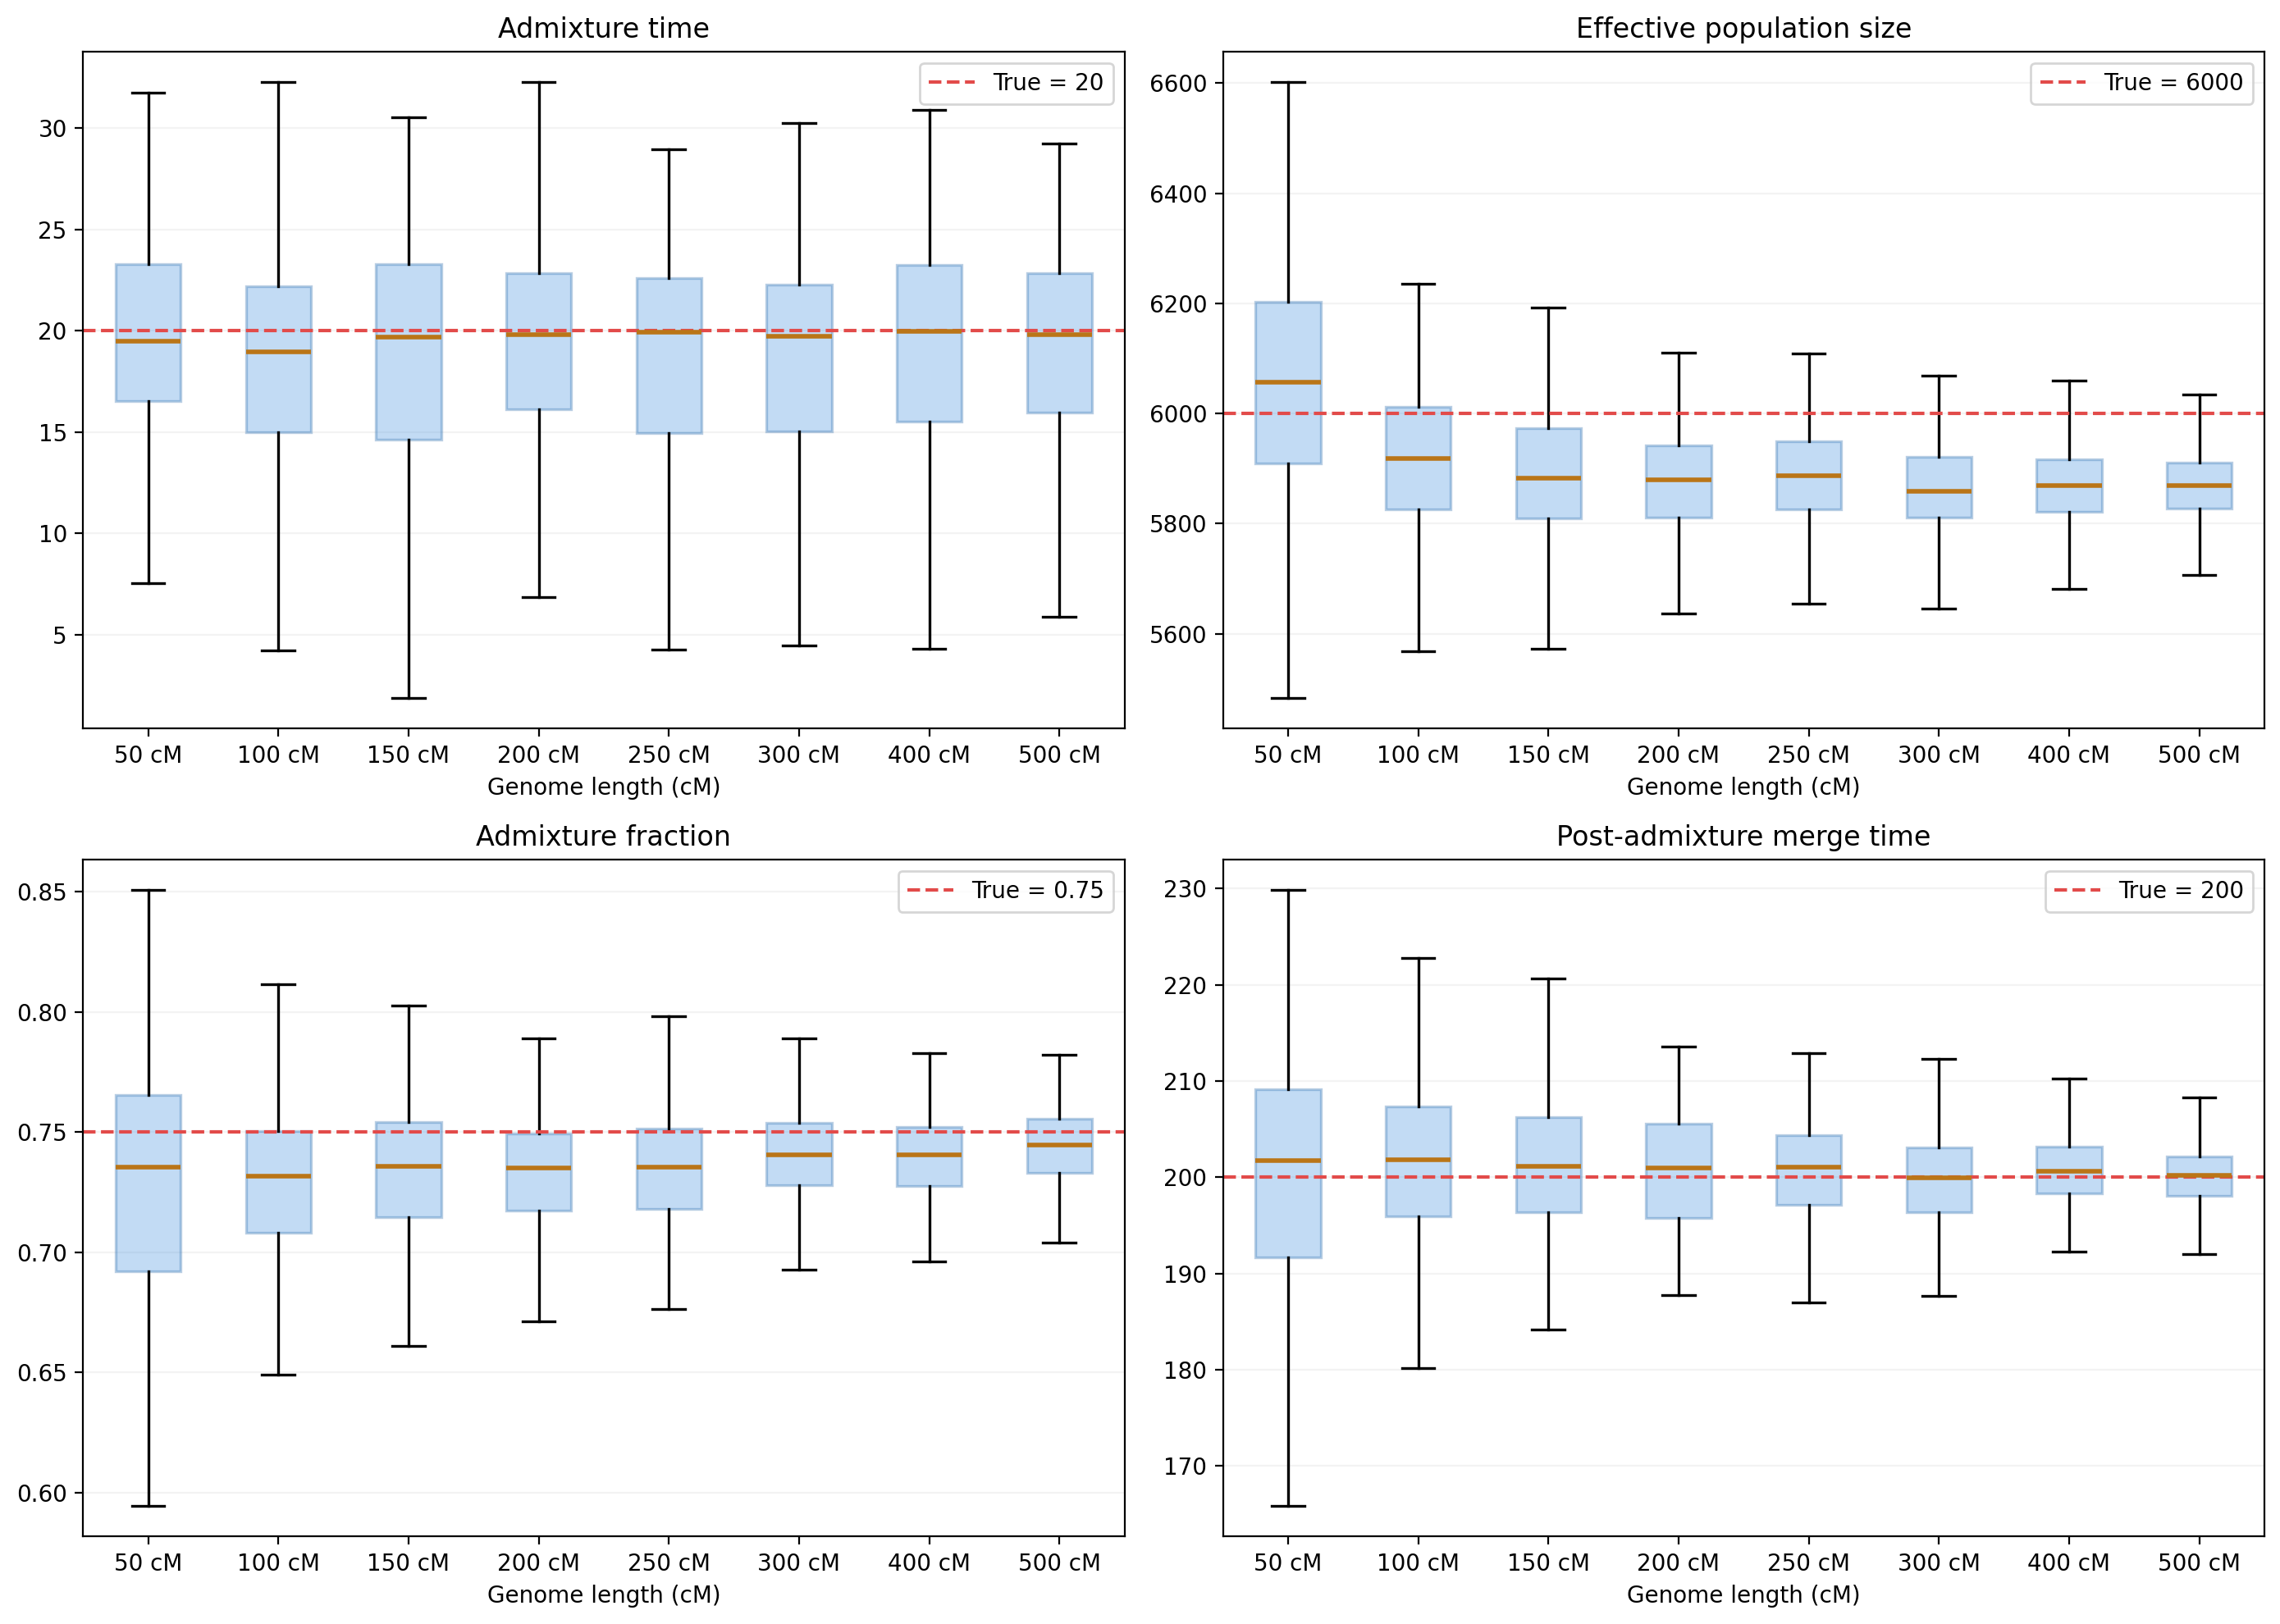
\includegraphics[width=15cm]{nfixed_parameters.png}
		\caption{Posterior estimation for uniform Ne
		}\label{fig:nfixed_parameters}
	\end{figure}

\cref{fig:nfixed_parameters} shows the posterior estimates of the four free
parameters (admixture time, effective population size, admixture fraction, and
the post-admixture merge time) as a function of the resampled genome length. As
the amount of data grows the posteriors concentrate around the truth: the
admixture time and fraction are recovered first (they are driven by the abundant
long IBD signal), while the effective population size and the deeper merge time
need more data to stabilize. This confirms that the IBD likelihood and the
zero-observation adjustment of \cref{sec:zero} together identify the recent part
of the history with modest amounts of genome.

\begin{figure}[!htbp]
    \centering
	    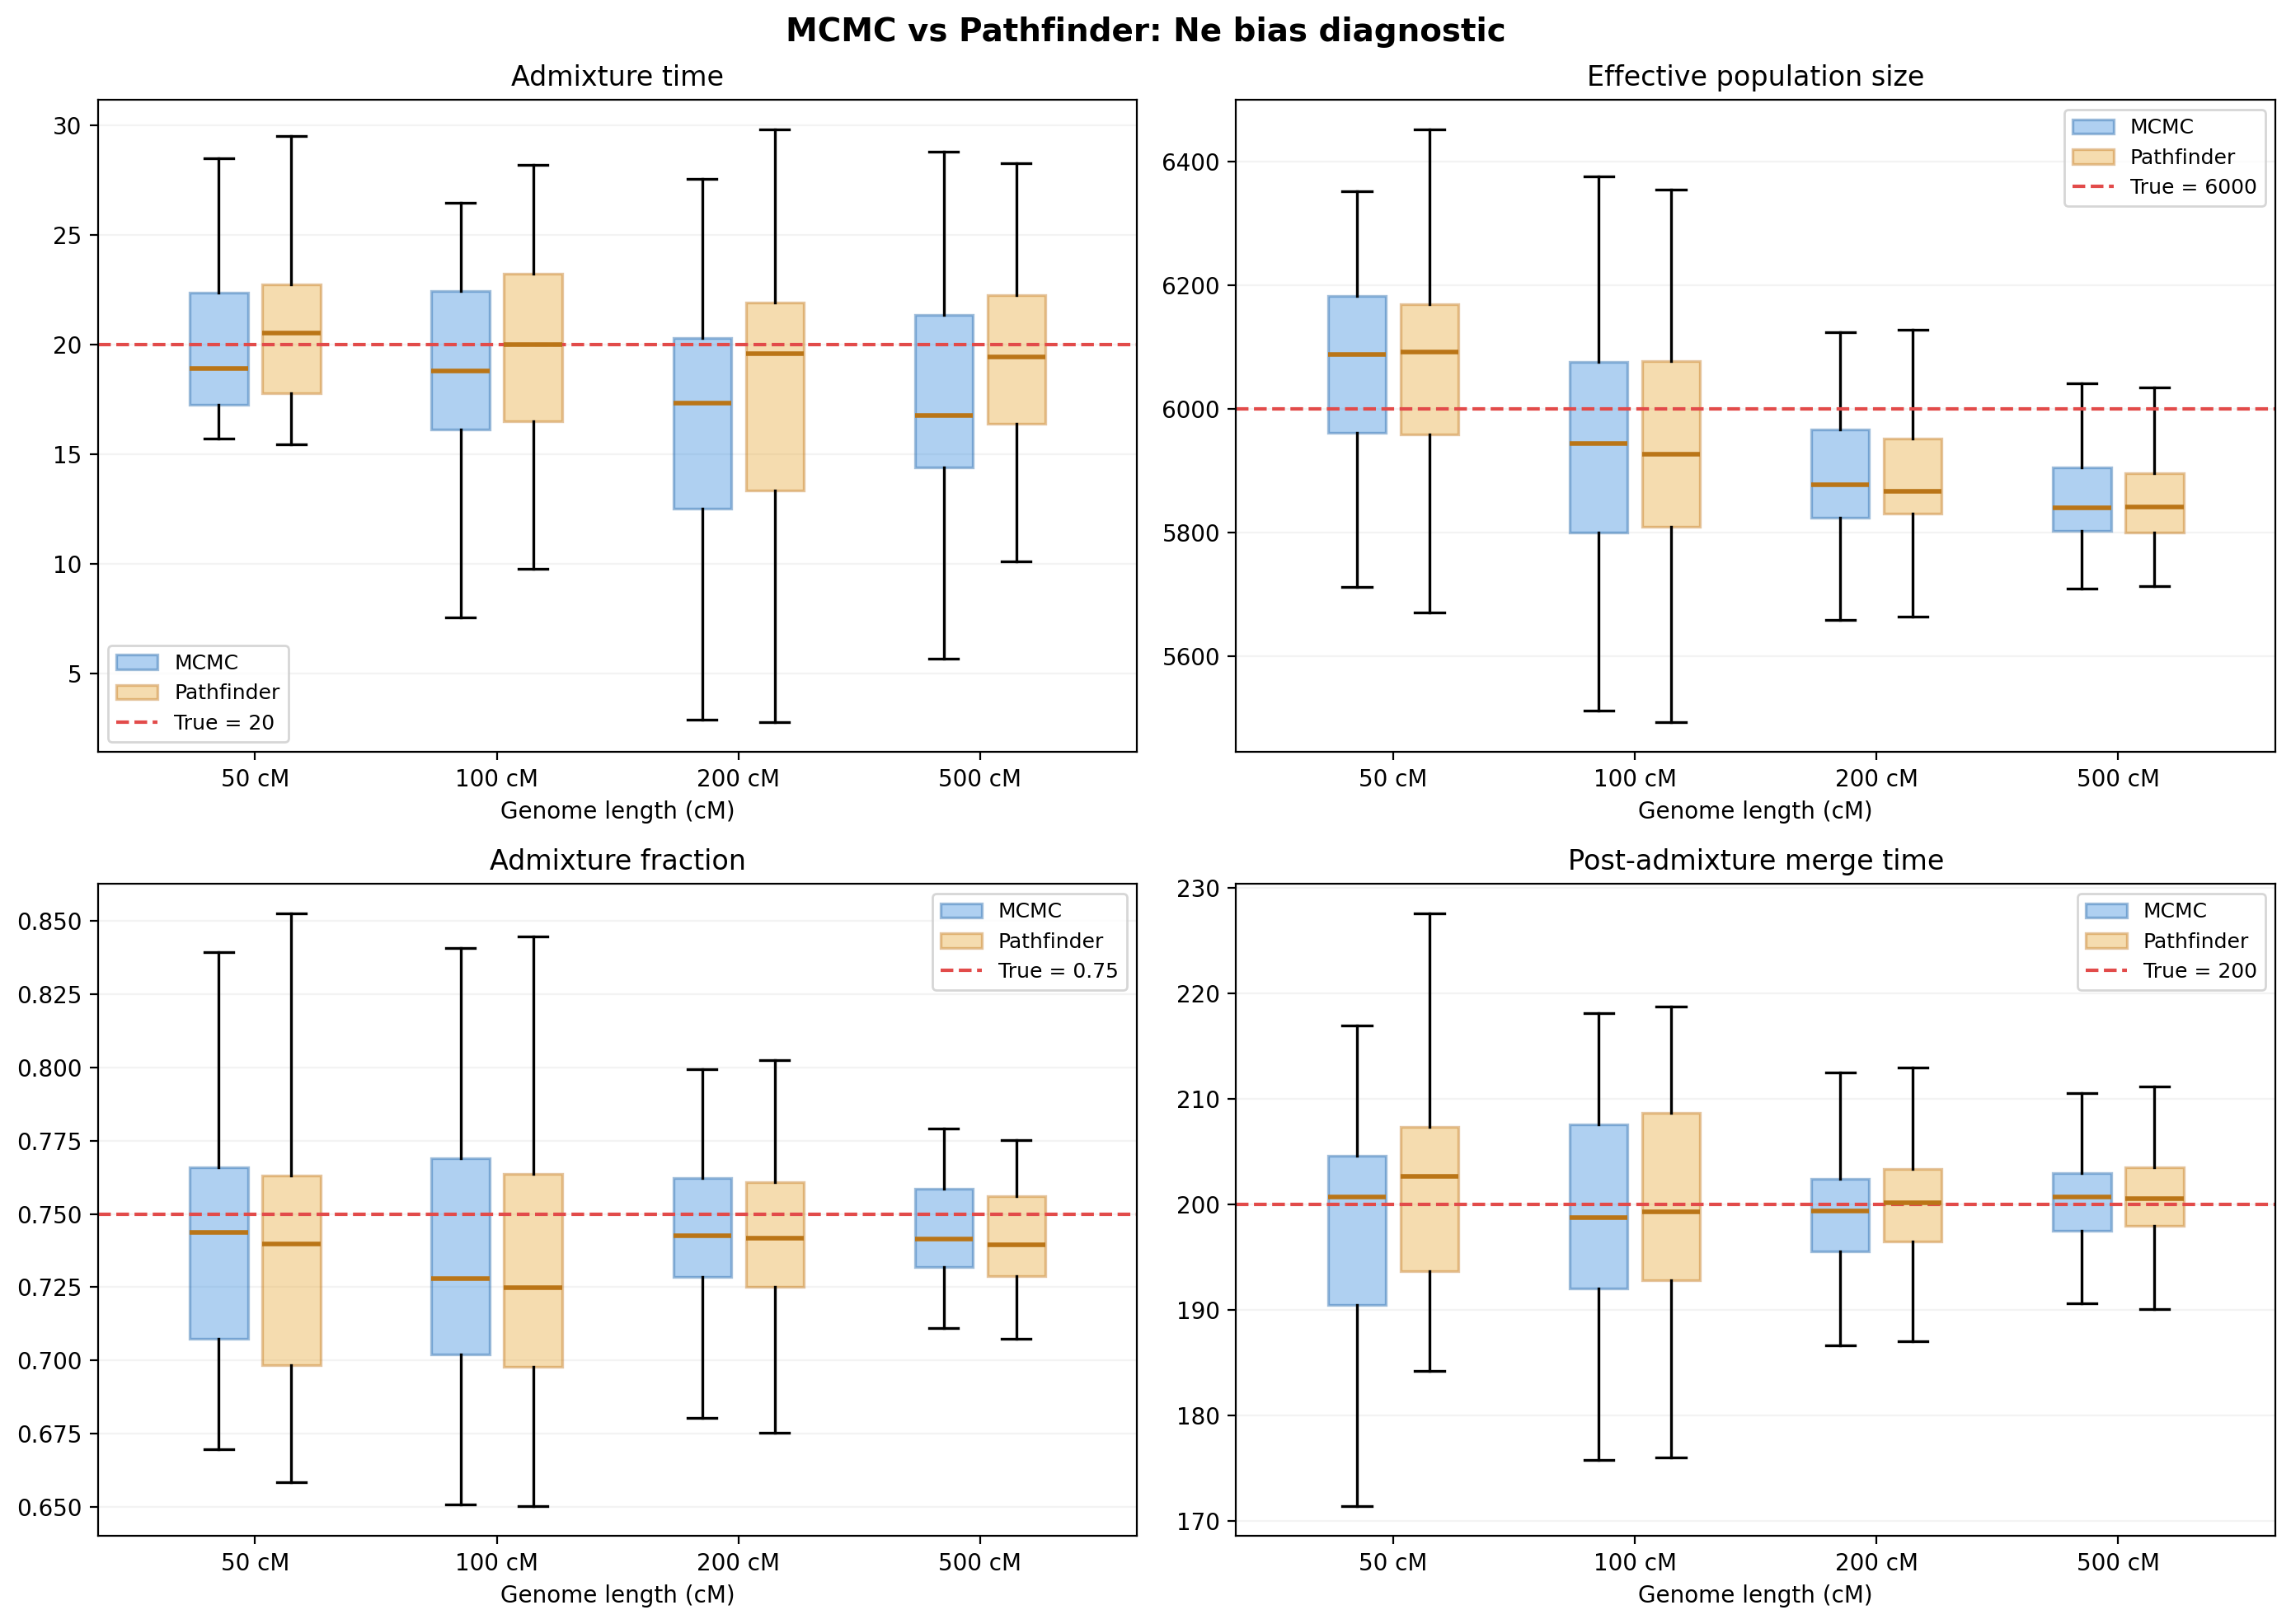
\includegraphics[width=15cm]{mcmc_vi_comparison.png}
		\caption{Bias and efficiency comparison for MCMC and Variational inference
		}\label{fig:mcmc_vi_comparison}
	\end{figure}

Because the variational engine is what makes the large model-selection sweeps
feasible, we check that it does not distort the inference. \cref{fig:mcmc_vi_comparison}
compares full Hamiltonian Monte Carlo against \texttt{pathfinder} on the same
resampled IBD data. The two agree closely on the point estimates; the main
discrepancy is a small ($\sim$2.5\%) downward bias in the effective population
size under the variational approximation, which shrinks with more data and is the
expected price of the Gaussian posterior approximation. Given the order-of-magnitude
speed-up, we adopt the variational engine for the topology-selection experiments
and treat MCMC as the reference for the parameter-recovery claims.
\subsubsection{Two Admixture Events: Recent vs. Ancient}
To probe whether the two data modalities carry the complementary signals
predicted in \cref{sec:framework,sec:snp}, we build a four-leaf topology
($a,b,c,d$, all sizes uniform at $N=10000$ haploid) that contains both a
\emph{recent} admixture and an \emph{ancient} one. The recent event is an
admixture-through-$b$ on lineage $a$ (split at $t=10$, merge of the donor branch
into $b$ at $t=55$, loop closing at $t=75$, mixing $\alpha=0.5$); the ancient
event is a $70\%/30\%$ admixture on lineage $c$ at $t=500$. The remaining merges
occur at $t=700,900$ and the root at $t=1000$.

\begin{figure}[!htbp]
    \centering
        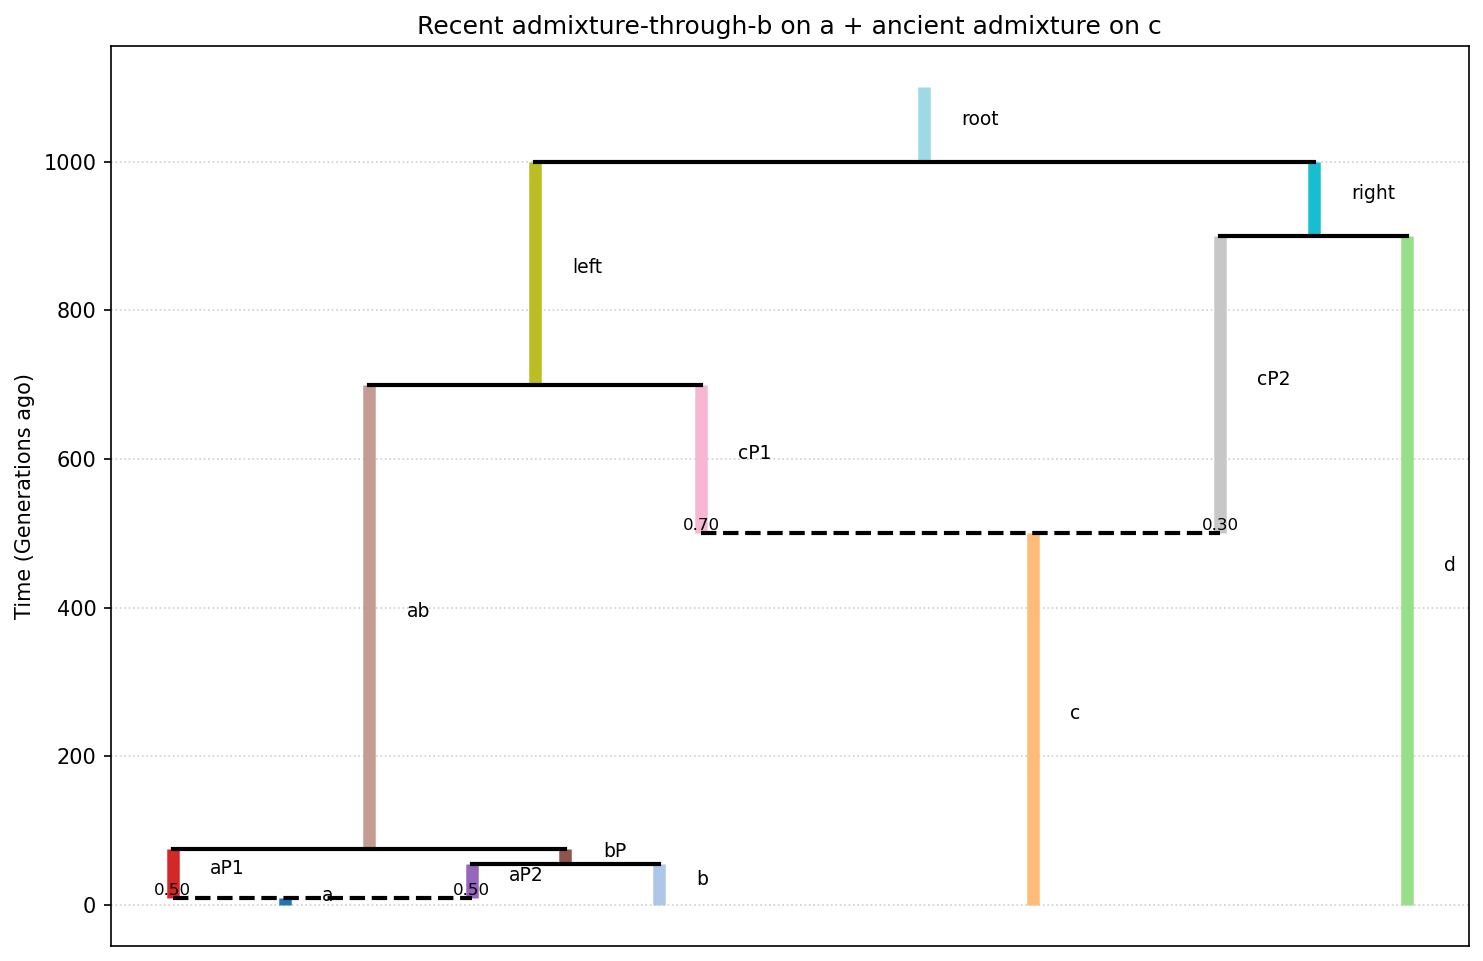
\includegraphics[width=14cm]{topology_sim2.png}
        \caption{True topology for the two-admixture experiment: a recent
        admixture-through-$b$ loop on lineage $a$ (split at $t=10$, donor branch
        merging into $b$ at $t=55$, loop closing at $t=75$, $\alpha=0.5$;
        dashed line = admixture) together with an ancient $70\%/30\%$ admixture
        on lineage $c$ at $t=500$. All effective sizes uniform at $N=10000$
        (haploid).}\label{fig:topology_sim2}
    \end{figure}

We fit three candidate topologies (\cref{fig:topology_sim2} is the true one) to
the same data: the true topology
($\text{T}_{\text{true}}$, both events), an alternative with the recent admixture
removed ($\text{T}_{\text{alt1}}$, ancient only), and one with the ancient
admixture removed ($\text{T}_{\text{alt2}}$, recent only). Each is fitted with the
IBD-only, SNP-only, and Mixed models over a grid of genome lengths
($50$--$1000$ cM), with $100$ resampled replicates each, and we record the ELBO
and the recovered parameters. The diagnostic is the sign of
$\Delta\text{ELBO}(\text{true}-\text{alt})$: a positive value means the data favor
keeping the corresponding event.

The design encodes a clear prediction. The IBD-only model should detect the
\emph{recent} admixture, $\Delta\text{ELBO}(\text{true}-\text{alt1})>0$, while
being essentially blind to the ancient one,
$\Delta\text{ELBO}(\text{true}-\text{alt2})\approx 0$. The SNP-only model should
show the mirror image: blind to the recent event but detecting the ancient one
through the $f$-statistic structure of the covariance. The Mixed model should
inherit both abilities.

\cref{fig:sim2_dELBO} confirms this division of labor. In the top row
($\Delta\text{ELBO}(\text{true}-\text{alt1})$, the recent-admixture test) the
IBD-only and Mixed models climb steadily above zero as the genome lengthens,
while the SNP-only model hovers around zero --- long shared segments reveal the
recent loop, $f$-statistics do not. The bottom row
($\Delta\text{ELBO}(\text{true}-\text{alt2})$, the ancient-admixture test)
is the mirror image: SNP-only and Mixed grow strongly positive (the SNP signal is
by far the largest, note the axis scale) while IBD-only stays near zero. The
Mixed model is the only one positive in \emph{both} rows, i.e. the only model
that recovers the full history. \cref{fig:sim2_params} tells the same story at the
level of individual parameters: the recent split time, the two recent merge
times, and the recent admixture fraction are recovered by IBD and Mixed (and
missed by SNP), whereas the ancient admixture time and fraction are recovered by
SNP and Mixed (and missed by IBD).

\begin{figure}[!htbp]
    \centering
        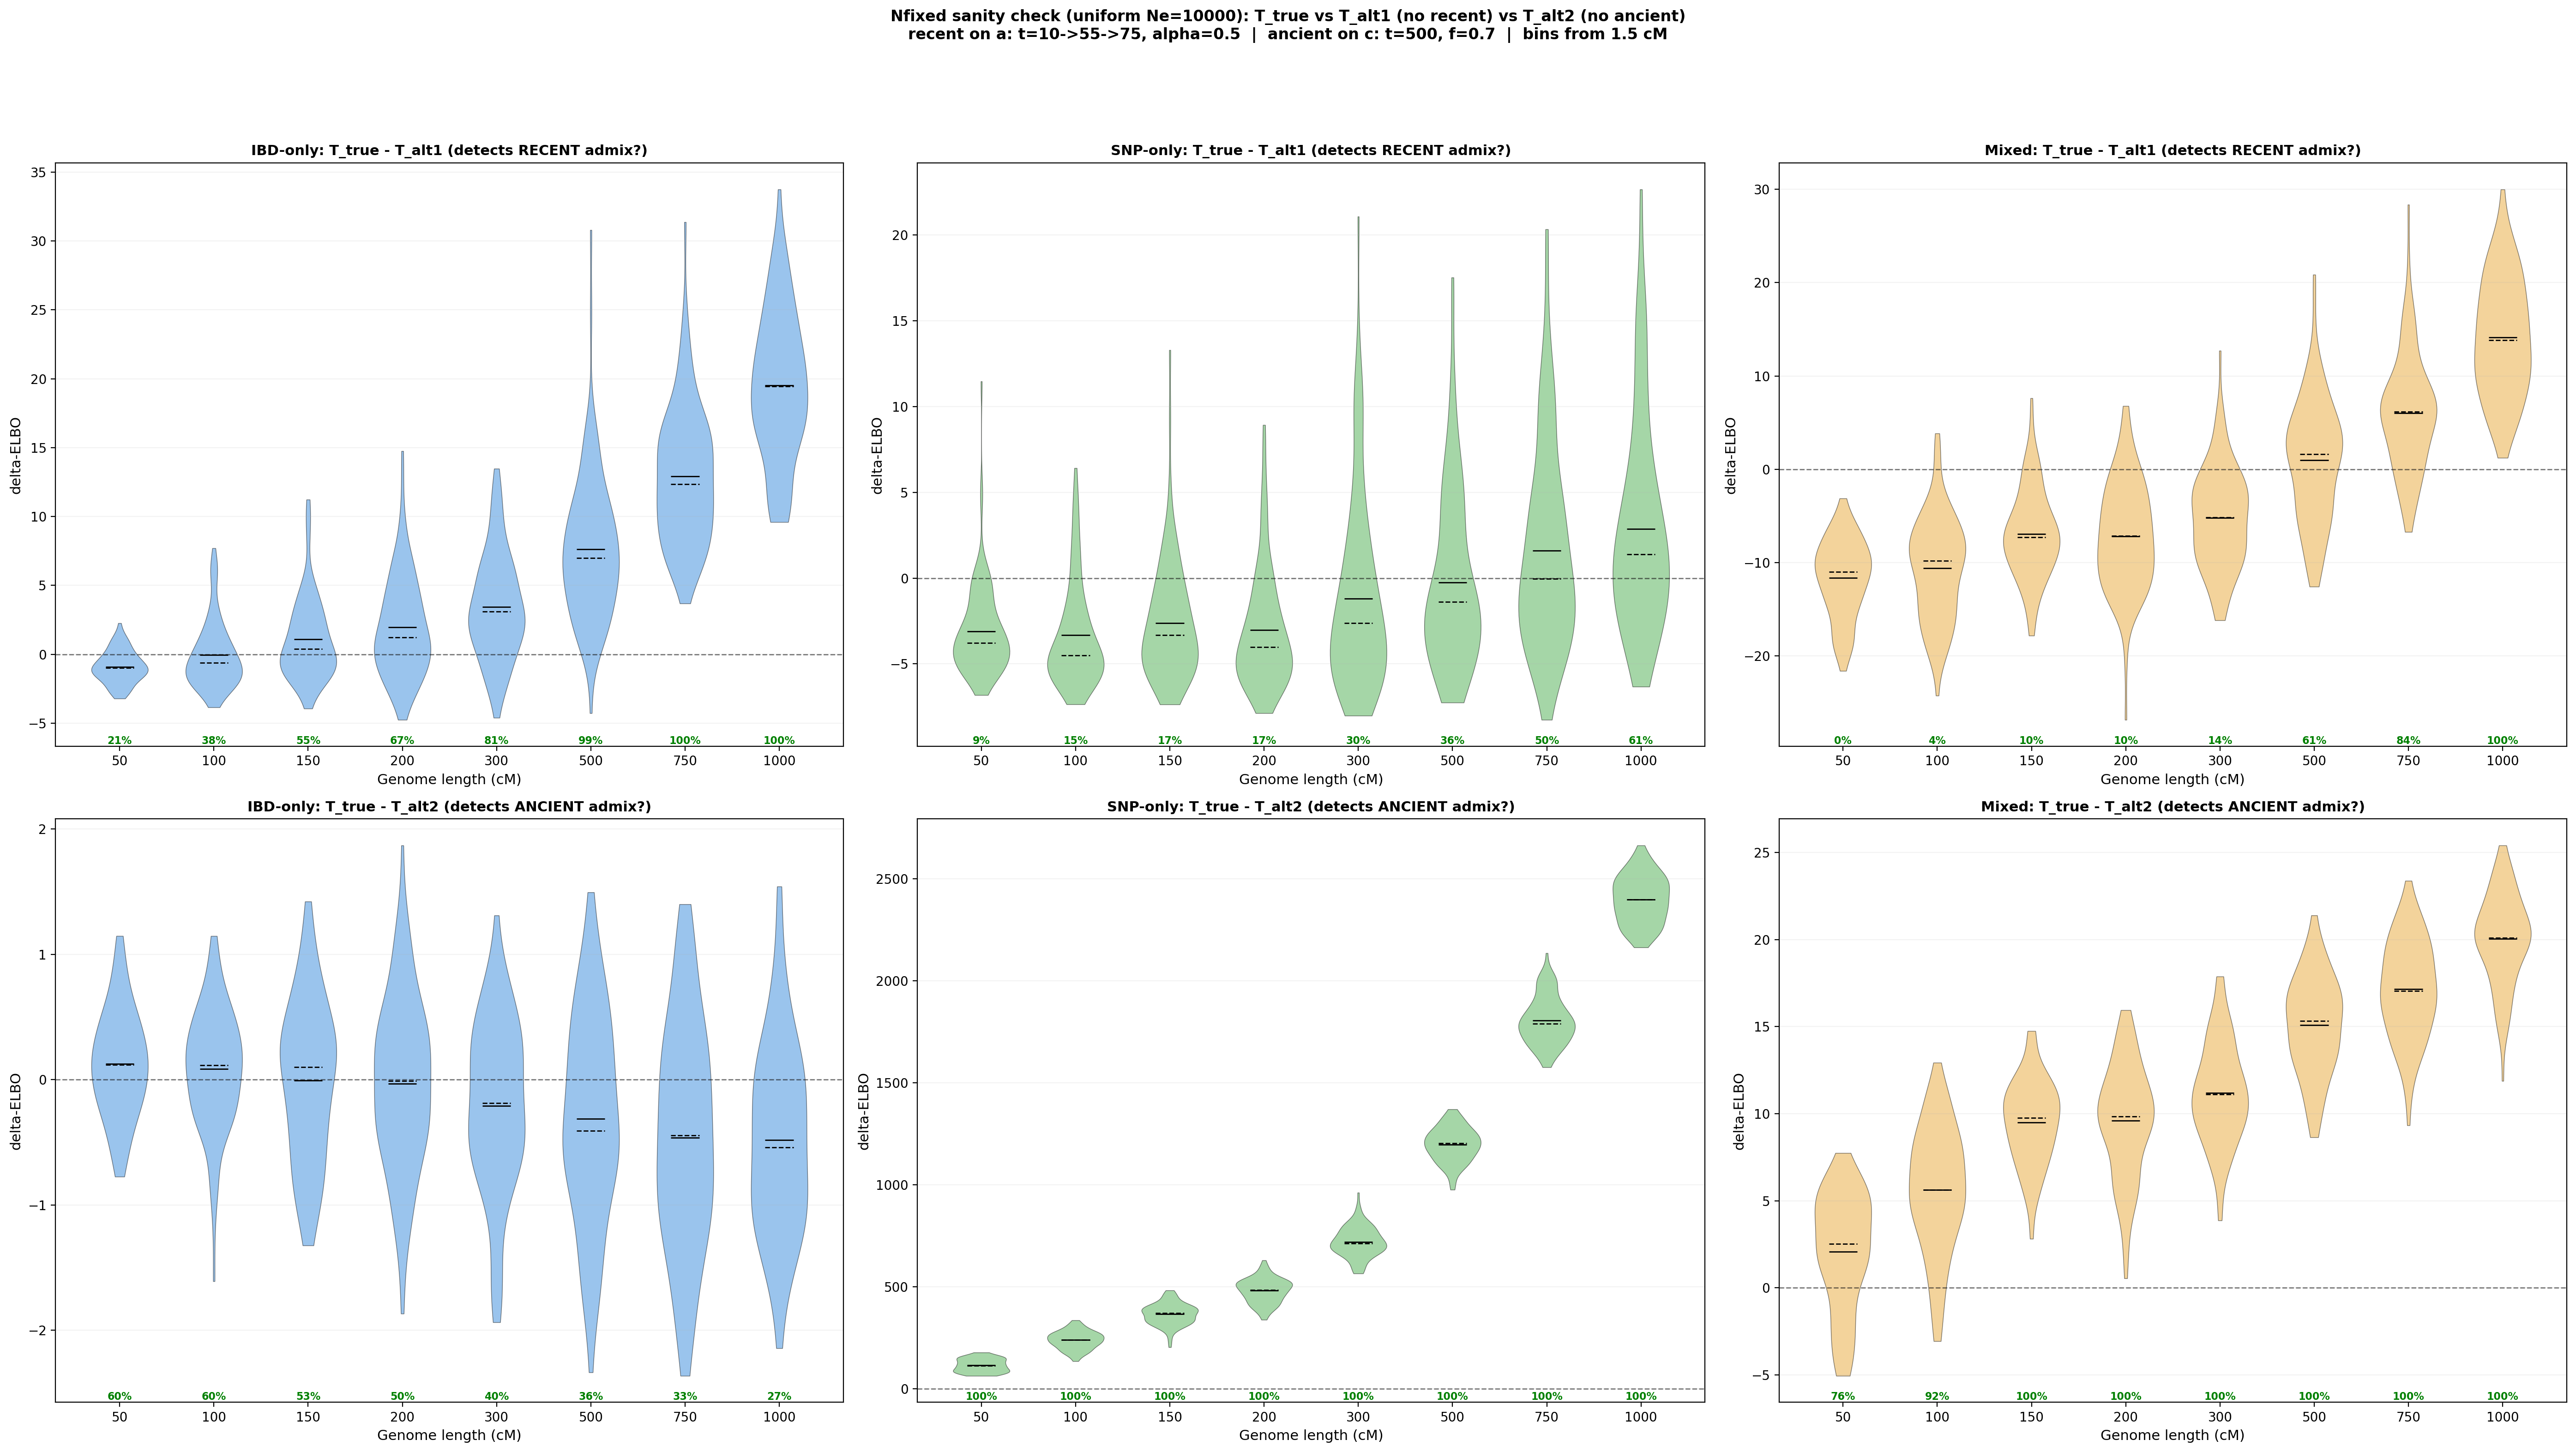
\includegraphics[width=\textwidth]{sim2_dELBO_trueibd.png}
        \caption{$\Delta\text{ELBO}$ versus genome length for the two-admixture
        experiment, using \textbf{true (tree-sequence) IBD}. Columns: IBD-only
        (blue), SNP-only (green), Mixed (orange). Top row: $\text{true}-\text{alt1}$
        (detects the recent admixture). Bottom row: $\text{true}-\text{alt2}$
        (detects the ancient admixture). Violins are over $100$ resampled
        replicates; the dashed line marks zero.}\label{fig:sim2_dELBO}
    \end{figure}

\begin{figure}[!htbp]
    \centering
        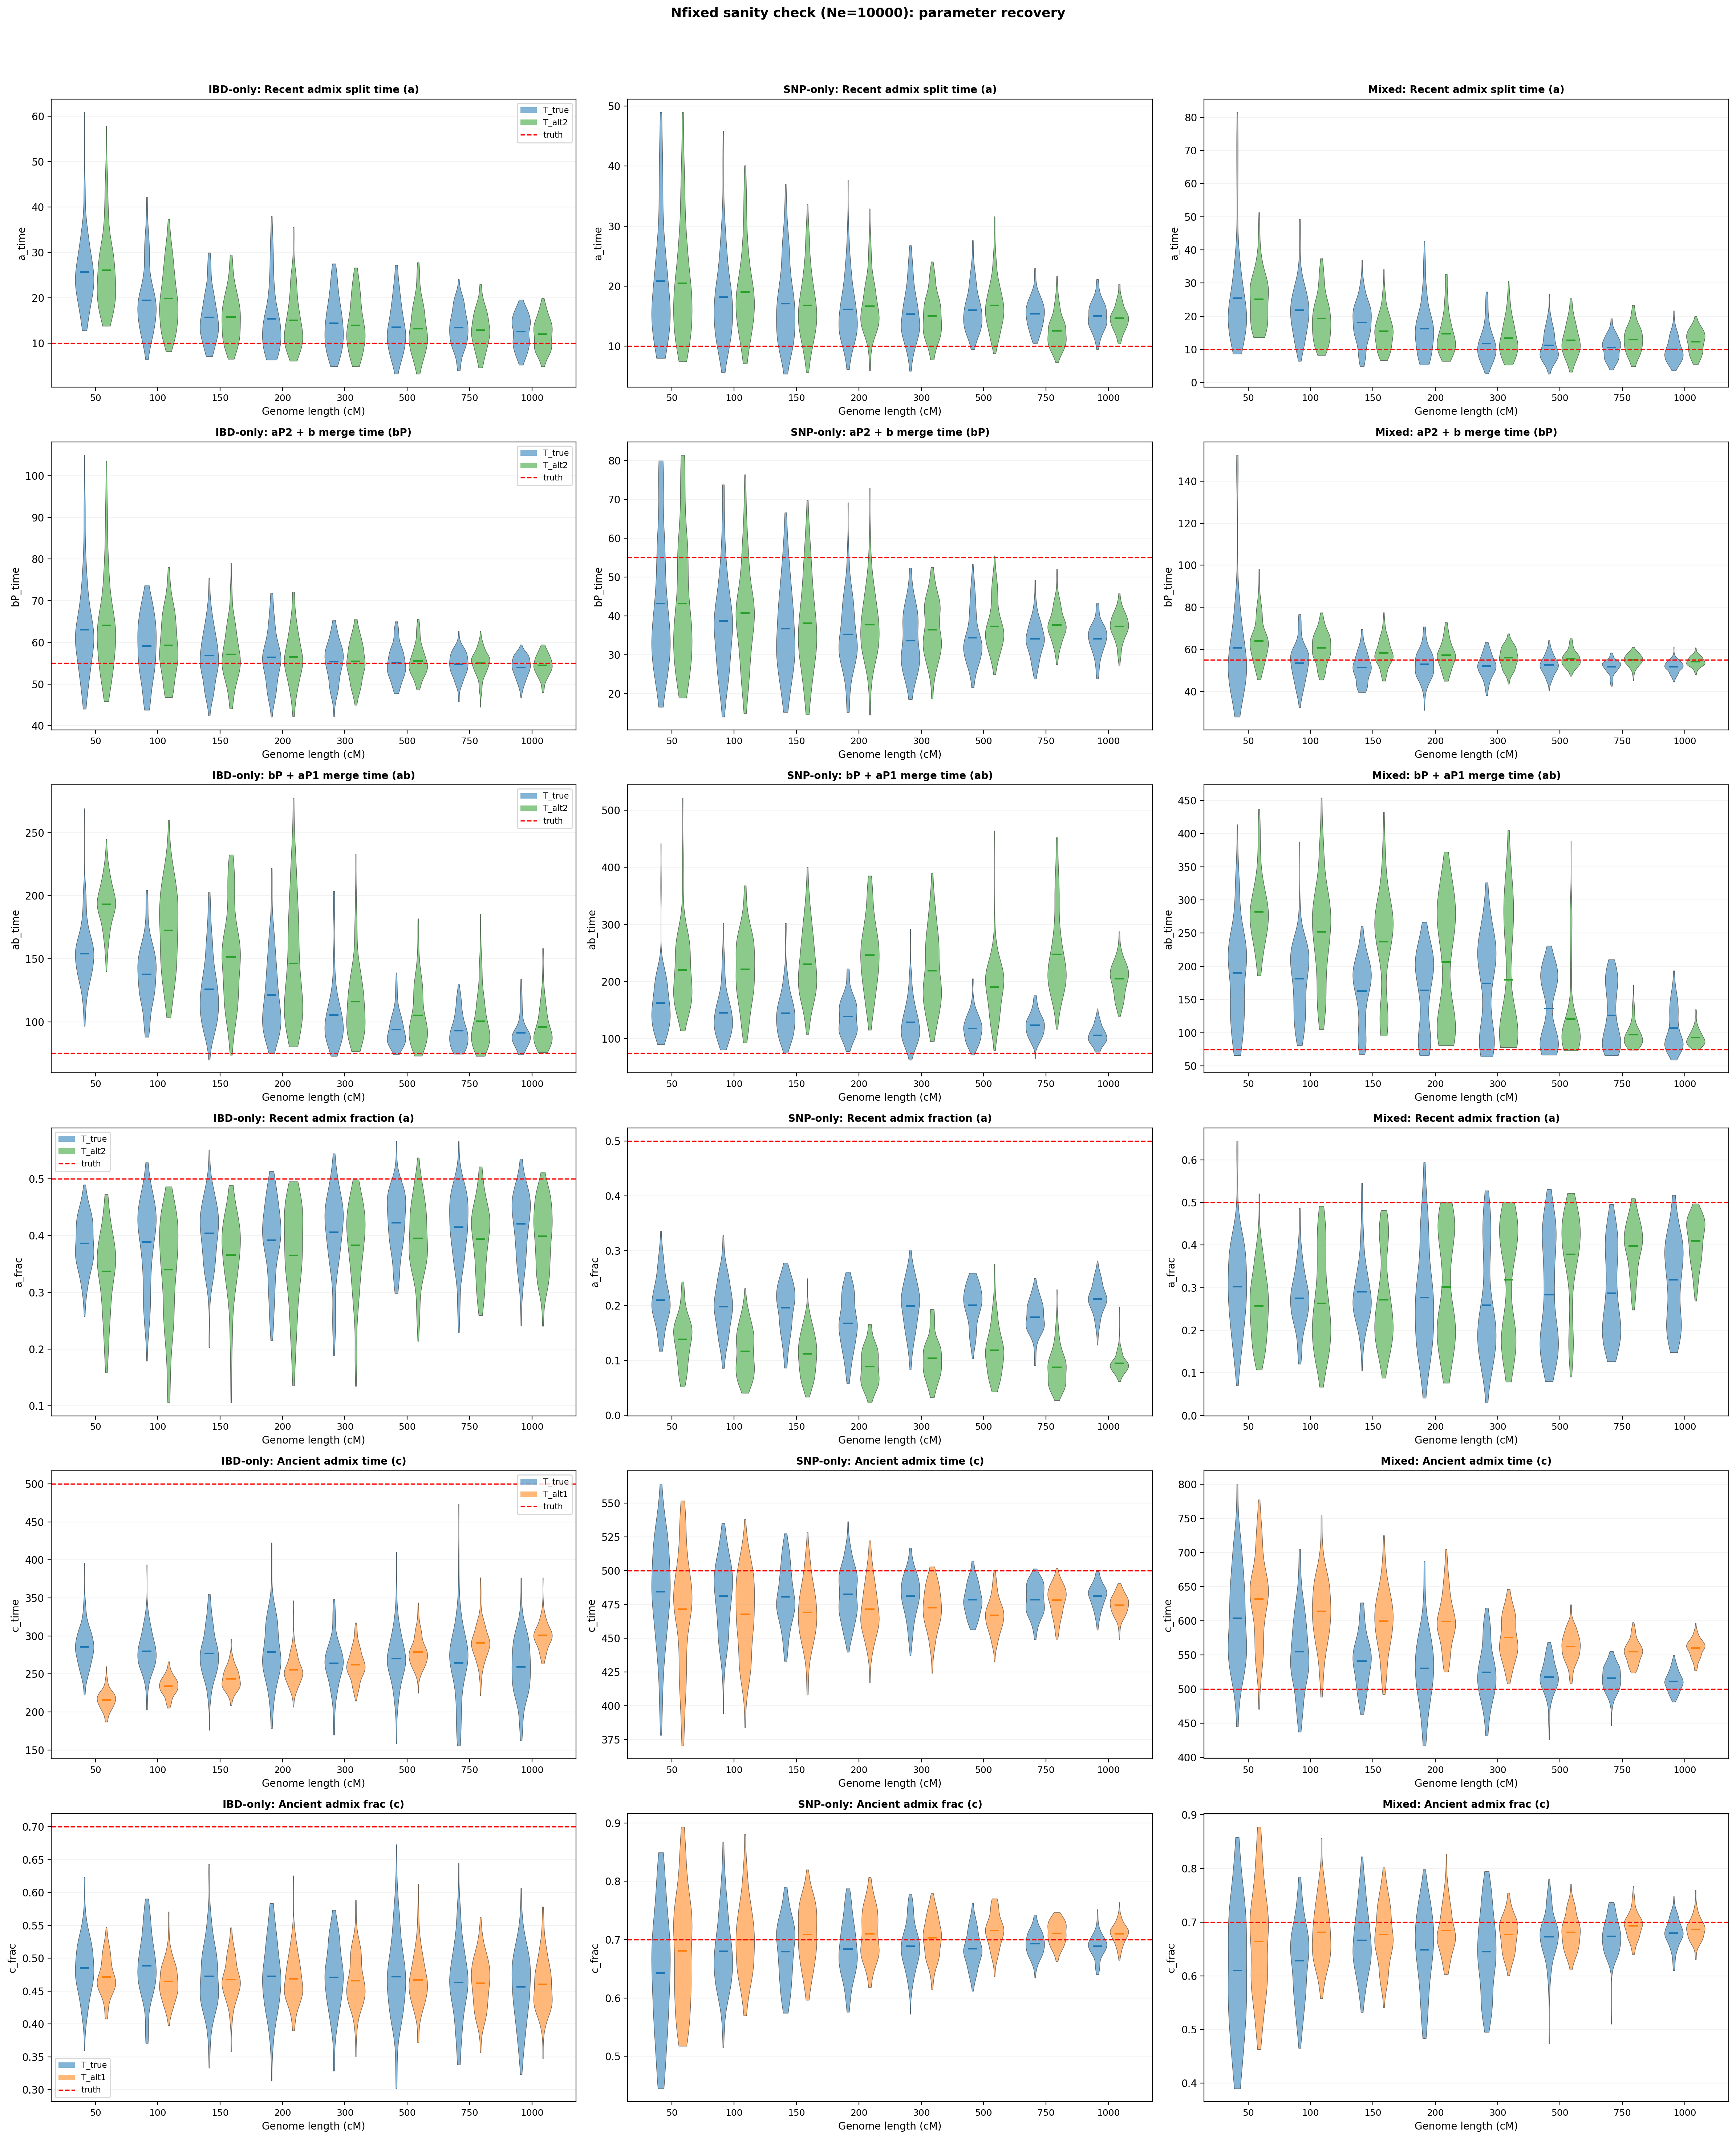
\includegraphics[width=\textwidth]{sim2_params_trueibd.png}
        \caption{Parameter recovery for the two-admixture experiment (true IBD).
        Rows are the six event parameters; columns are the IBD-only, SNP-only and
        Mixed models; red lines are the simulated truth. Recent-event parameters
        are recovered by IBD/Mixed, ancient-event parameters by
        SNP/Mixed.}\label{fig:sim2_params}
    \end{figure}

\paragraph{True IBD versus estimated IBD.}
The results above use the \emph{true} IBD segments, read directly from the
simulated tree sequence as spans of constant most-recent-common-ancestor. With
real data the IBD segments are not observed: they must be \emph{estimated} from
genotypes by an IBD caller, which introduces phasing errors, a detection-length
threshold, and boundary noise that the tree-sequence ground truth does not have.
To check that our conclusions survive this, we repeat the identical experiment but
replace the tree-sequence segments with segments called by \texttt{Hap-IBD} run
on the simulated genotypes (VCF plus a uniform genetic map); everything
downstream --- binning, block pooling, jackknife variance, and inference --- is
unchanged. \cref{fig:sim2_dELBO_hapibd,fig:sim2_params_hapibd} show that the
estimated-IBD pipeline reproduces the same qualitative picture as the true-IBD
pipeline: IBD/Mixed detect the recent event, SNP/Mixed detect the ancient event,
and the parameter recovery degrades only modestly (slightly noisier violins and a
mild attenuation at short genome lengths, where few long segments survive the
caller's length threshold). This is the key robustness check: the recent-versus-
ancient division of labor is a property of the data, not an artifact of having
access to the exact genealogy.

\begin{figure}[!htbp]
    \centering
        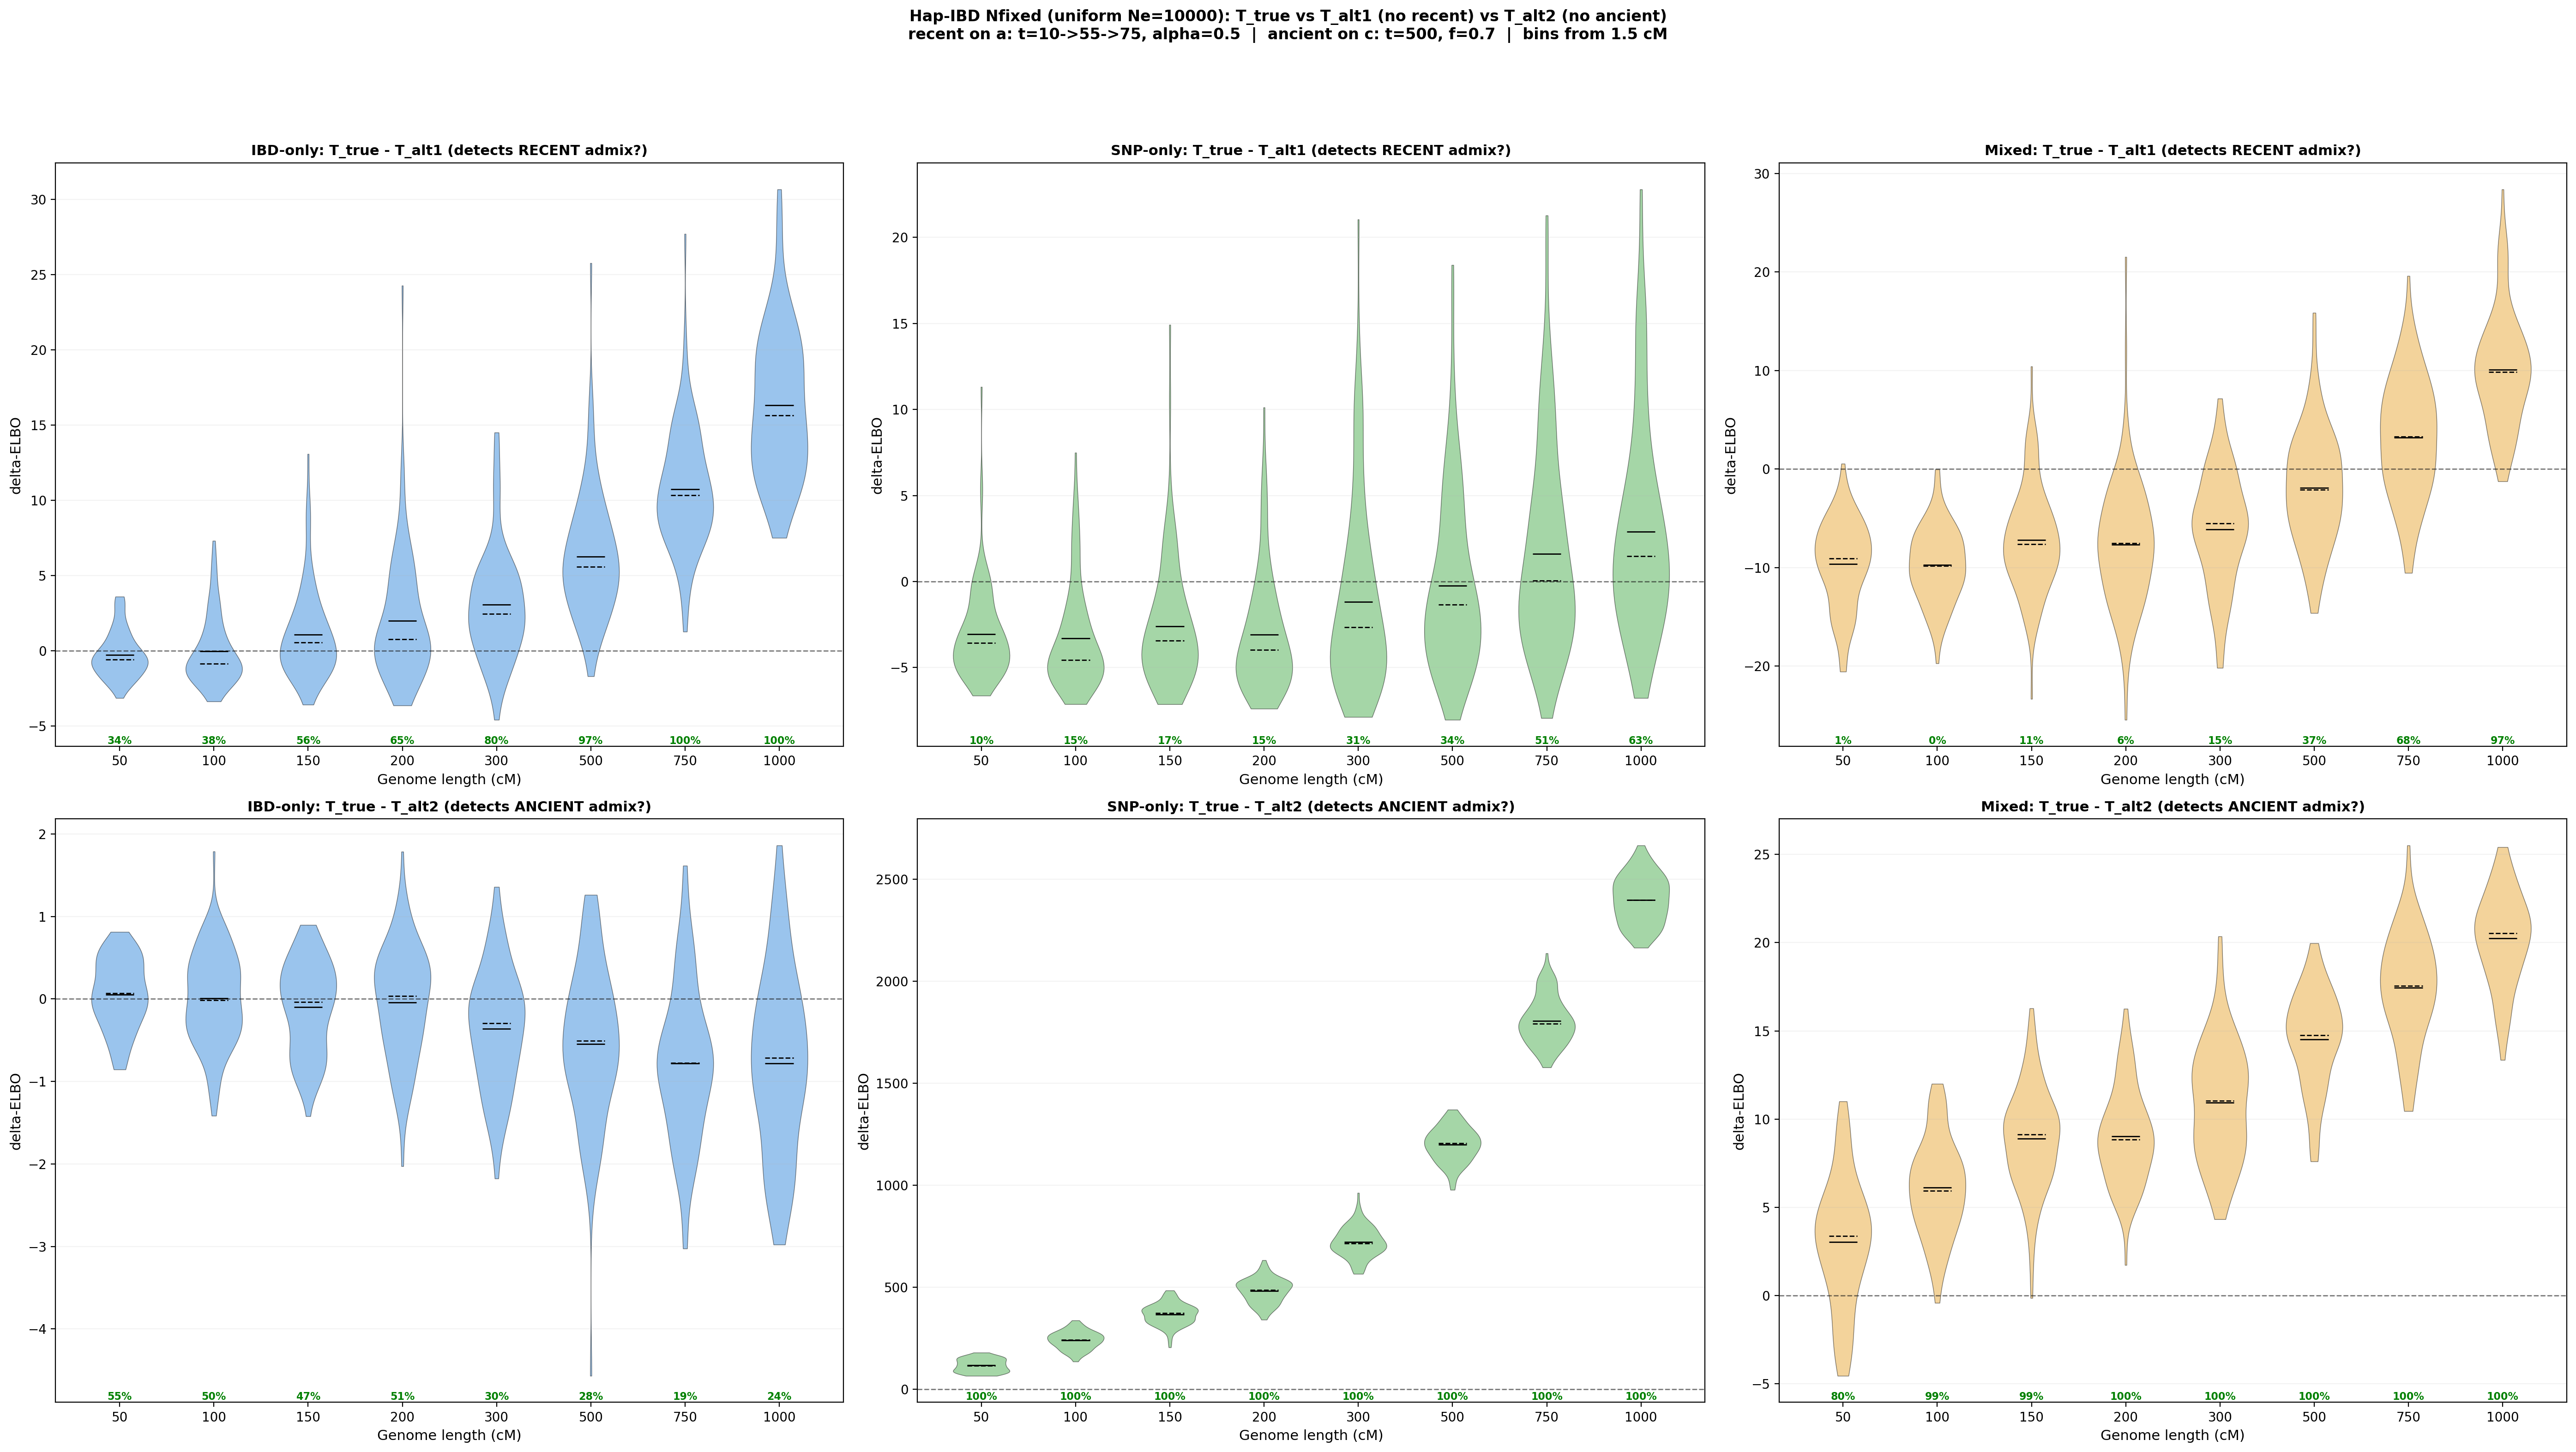
\includegraphics[width=\textwidth]{sim2_dELBO_hapibd.png}
        \caption{As \cref{fig:sim2_dELBO} but with IBD segments
        \textbf{estimated by \texttt{Hap-IBD}} from genotypes rather than read from
        the tree sequence. The same detection pattern survives realistic IBD
        calling.}\label{fig:sim2_dELBO_hapibd}
    \end{figure}

\begin{figure}[!htbp]
    \centering
        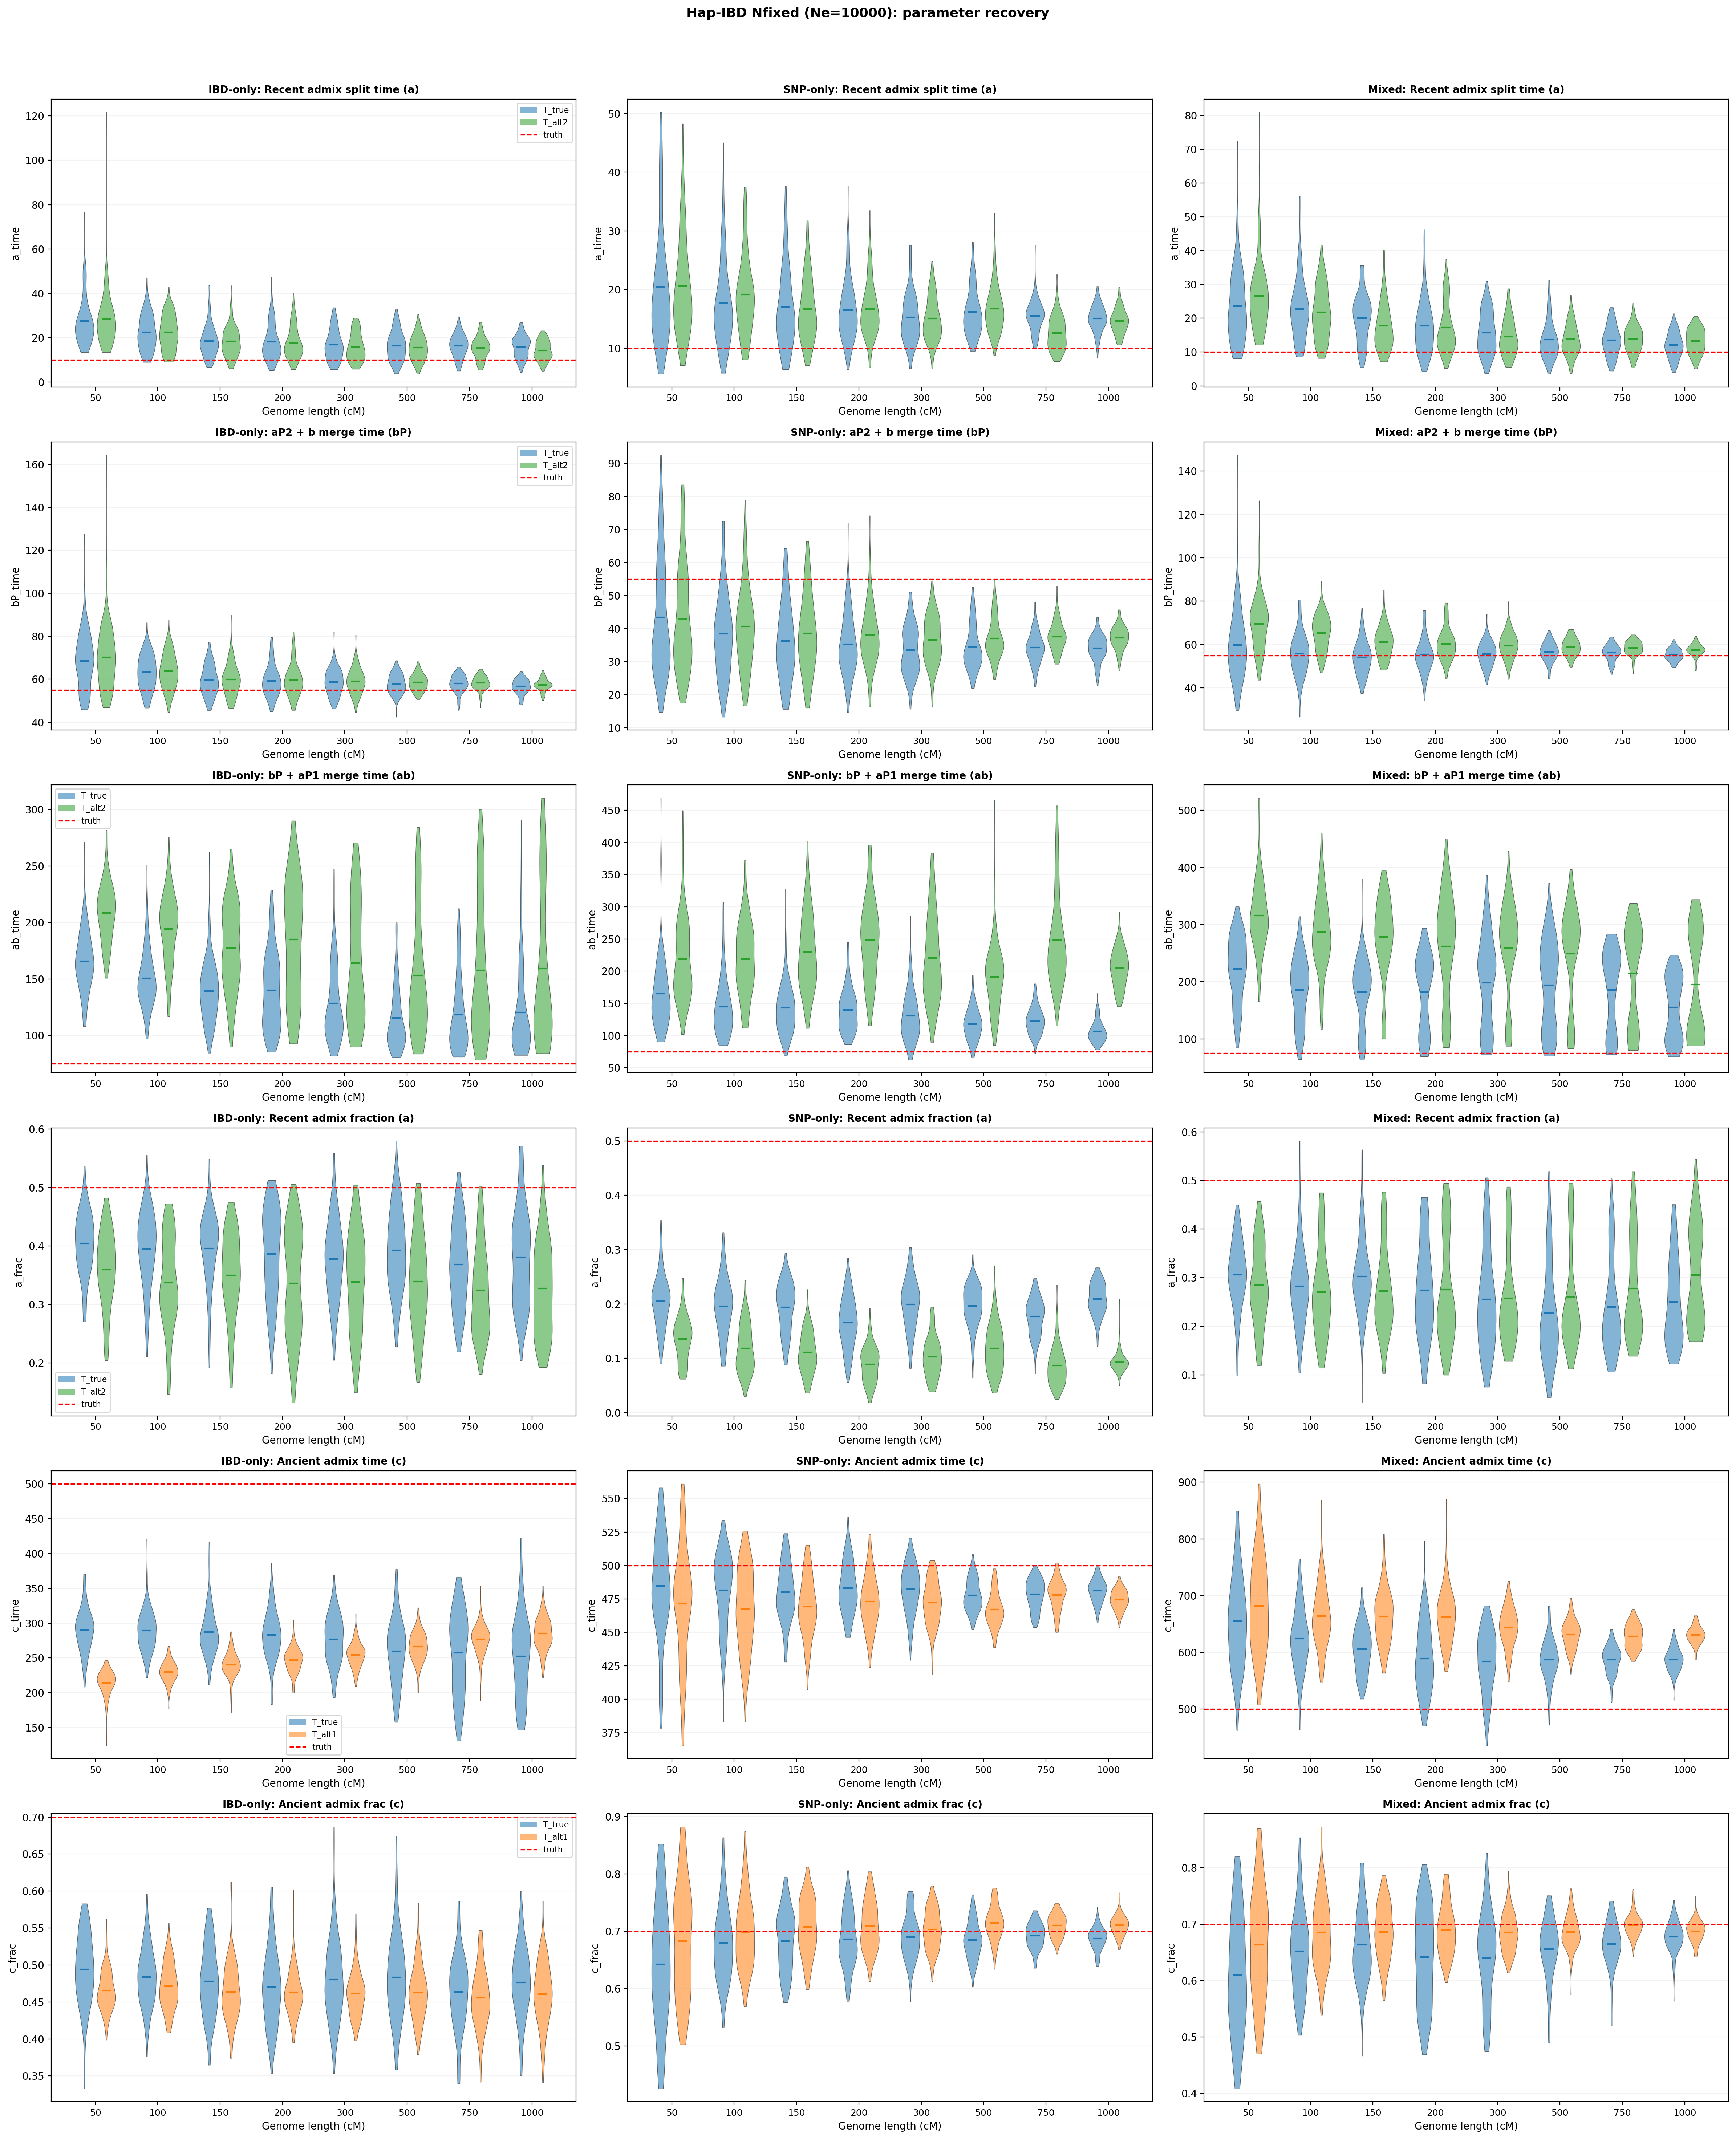
\includegraphics[width=\textwidth]{sim2_params_hapibd.png}
        \caption{Parameter recovery for the two-admixture experiment with
        \texttt{Hap-IBD}-estimated segments. Compare
        \cref{fig:sim2_params}.}\label{fig:sim2_params_hapibd}
    \end{figure}
\subsection{Pathfinder versus MCMC (HMC)}\label{sec:vi_vs_mcmc}
The whole simulation programme above relies on \texttt{pathfinder} variational
inference (\cref{sec:framework}) rather than full posterior sampling, because
each experiment fits hundreds of model$\times$topology$\times$replicate
combinations. Before trusting that choice we benchmark it against the gold
standard, full Hamiltonian Monte Carlo (HMC, as implemented by Stan's NUTS
sampler), on the one-admixture uniform-$N$ setup of \cref{fig:topology_example}.
We fit the same resampled IBD data with both engines over $100$ replicates at
each of five genome lengths; HMC is run with $4$ chains, $1000$ warm-up and
$2000$ sampling iterations per chain. The comparison has two parts: whether the
two engines \emph{agree} (bias of the posterior mean), and what that agreement
\emph{costs} (running time).

\cref{fig:mcmc_vi_comparison} already showed the per-parameter posterior
distributions side by side: the \texttt{pathfinder} and HMC boxes overlap almost
entirely, so the variational approximation is recovering essentially the same
posterior location and spread as the exact sampler. \cref{fig:mcmc_efficiency}
makes this quantitative and adds the cost axis. The first four panels plot the
bias of the posterior mean (as a percent of the true value) for the four free
parameters: the two engines track each other closely at every genome length, and
the residual biases --- a few-percent under-estimate of the admixture time and
fraction, a $\lesssim 2\%$ wobble in the effective size and the post-admixture
merge time --- are \emph{finite-data} effects shared by both methods, not
artifacts introduced by the variational approximation. In other words,
\texttt{pathfinder} adds negligible extra bias on top of HMC. The final panel is
the running time per replicate: HMC costs $\sim 60$--$110$ s and grows with the
amount of data, whereas \texttt{pathfinder} stays at $\sim 1$--$2$ s, a roughly
$50$--$100\times$ speed-up. This is what makes the large topology-selection sweeps
of \cref{sec:simstudy} feasible, and it justifies using \texttt{pathfinder}
throughout while reserving HMC as the reference for the parameter-recovery claims.

\begin{figure}[!htbp]
    \centering
        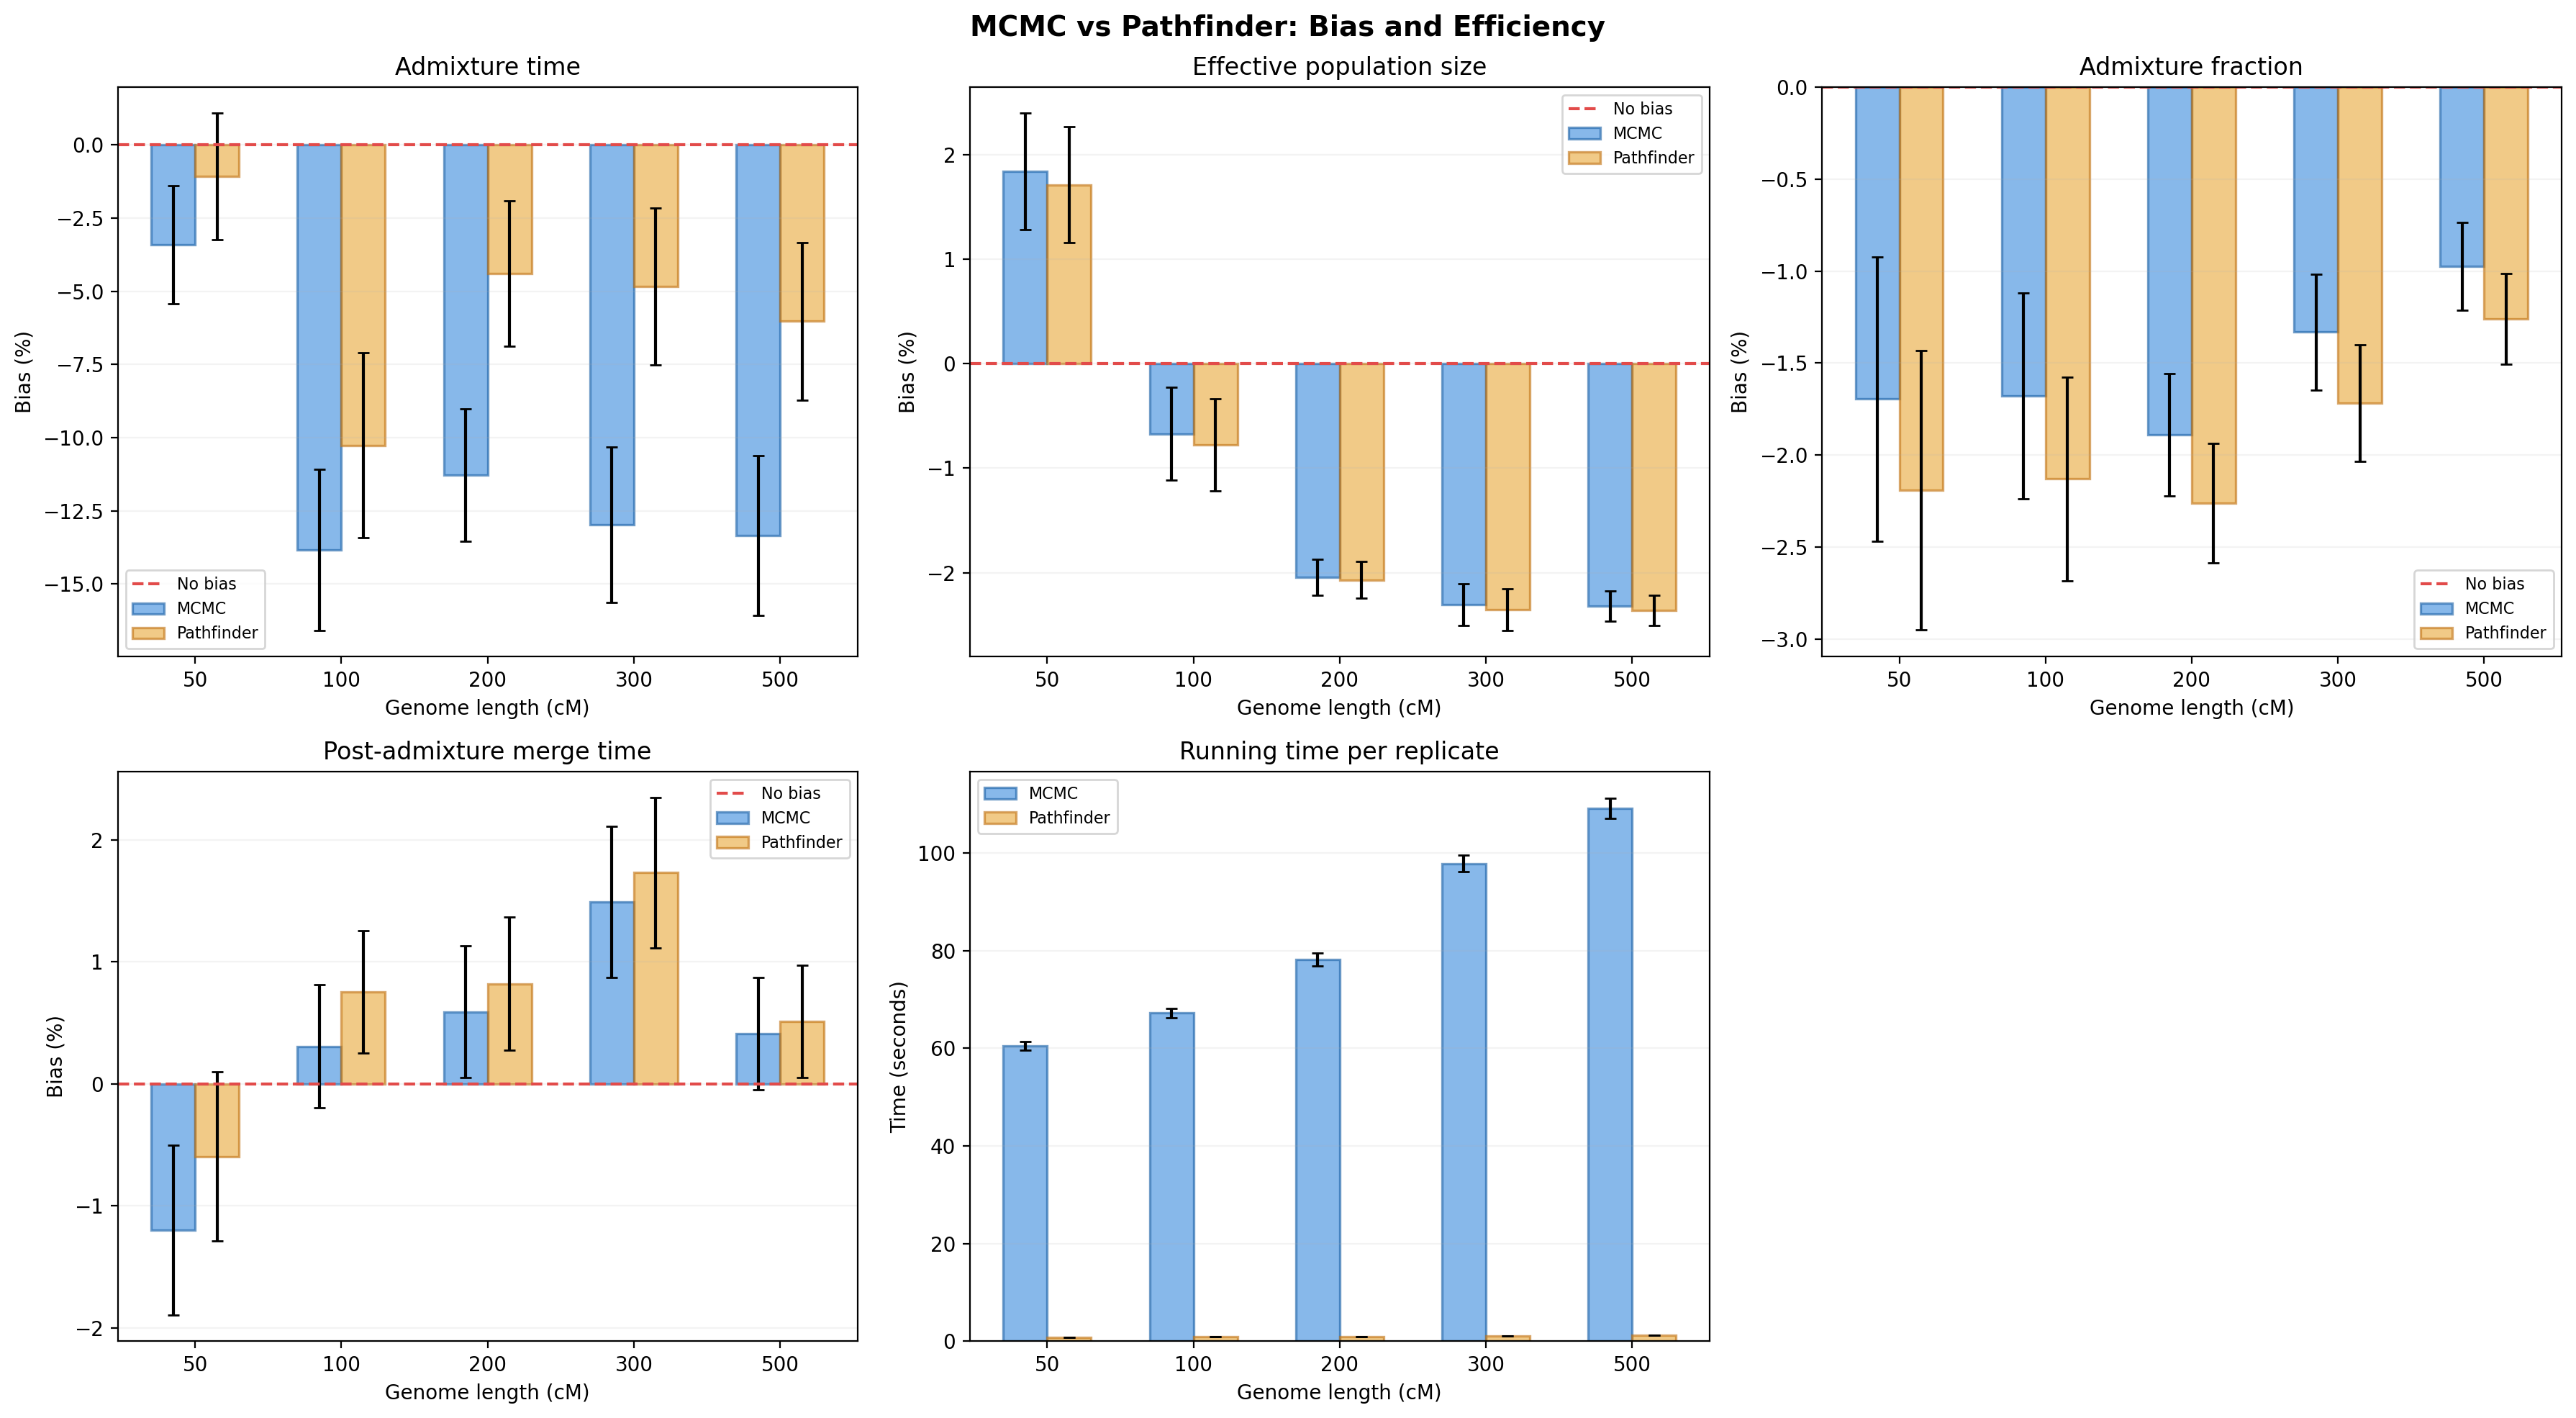
\includegraphics[width=\textwidth]{mcmc_pathfinder_bias_efficiency.png}
        \caption{Pathfinder versus MCMC (HMC): bias and efficiency. First four
        panels: bias of the posterior mean (percent of truth) for the admixture
        time, effective population size, admixture fraction and post-admixture
        merge time, versus genome length; blue = MCMC, orange = Pathfinder, red
        dashed = no bias. Last panel: running time per replicate, showing the
        $\sim$$50$--$100\times$ speed-up of Pathfinder over HMC. $100$ replicates
        per genome length.}\label{fig:mcmc_efficiency}
    \end{figure}
\subsection{Varying Effective Population Sizes}
The framework extends without modification to per-node effective sizes: the
recursion of \cref{alg:ibd} reads $N_a$ from a size vector instead of a single
scalar, and the SNP covariance uses the same per-node sizes in $\Delta t_e/N_a$.
The corresponding \texttt{Nvarying} models infer one size per population alongside
the times and admixture fractions. The added flexibility comes at the cost of
weaker identifiability: a recent branch's size and the duration of the epoch
trade off against each other in the IBD likelihood, so the per-node sizes are
recovered with larger uncertainty than the shared size of the uniform setting,
and longer genomes are required before the deep-node sizes are pinned down.

We illustrate the varying-$N$ regime with two five-population experiments that
both carry a recent and an old admixture but differ in whether the recent event
is resolvable: a \emph{success} case where the Mixed model beats both single-data
models on both events, and a \emph{failure} case that exposes a genuine
identifiability limit.

\subsubsection{Success: the Mixed model beats both single-data models}
The true topology (\cref{fig:topo_v2}) has a recent admixture on $b$ at $t=20$
($90\%$ from the $a$-side, $10\%$ from the $c$-side) and an old admixture on $d$
at $t=500$ ($70\%/30\%$), with non-uniform sizes ($N_b=N_d=5000$, all others
$15000$ haploid). As before, $\text{T}_{\text{alt1}}$ drops the recent event and
$\text{T}_{\text{alt2}}$ drops the old event. \cref{fig:dELBO_v2} shows that here
the data are rich enough that all three models eventually favor the true topology
on both axes (all violins climb above zero), but the Mixed model does so
\emph{earliest and most decisively} on both the recent test (top row) and the old
test (bottom row): it inherits the recent-admixture signal from IBD and the
old-admixture signal from SNP, and so dominates either single-data model. This is
the regime the composite likelihood is designed for --- each modality supplies
the event the other cannot see, and combining them strictly helps.

\begin{figure}[!htbp]
    \centering
        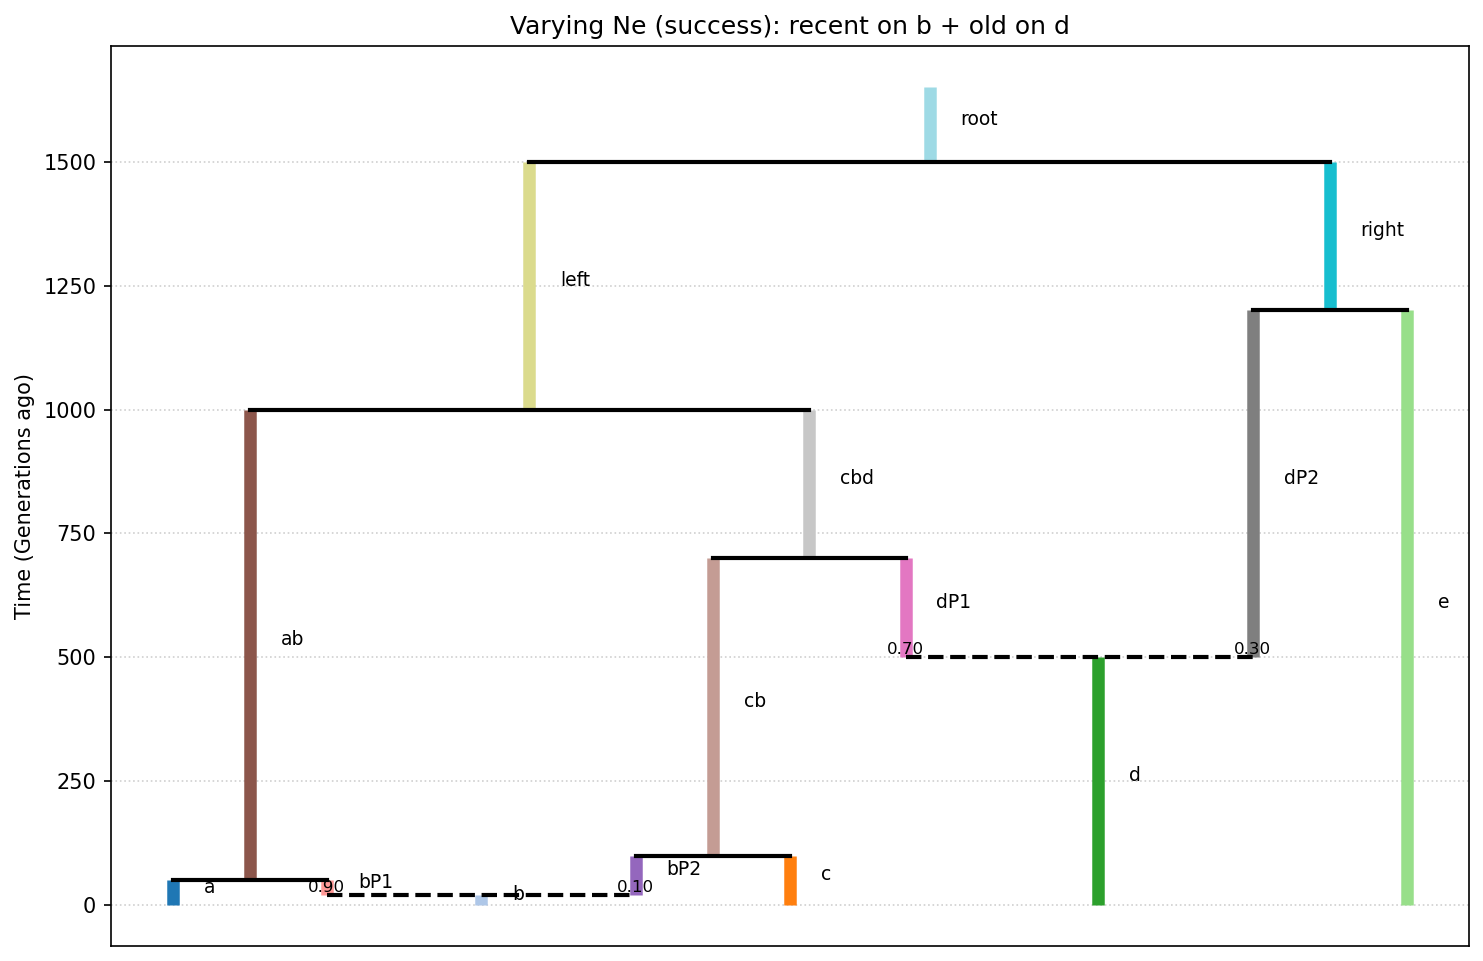
\includegraphics[width=13.5cm]{topology_mixed_v2.png}
        \caption{Varying-$N$ success case (true topology): recent admixture on
        $b$ ($t=20$, $90\%$/$10\%$) and old admixture on $d$ ($t=500$,
        $70\%$/$30\%$); $N_b=N_d=5000$, others $15000$
        (haploid).}\label{fig:topo_v2}
    \end{figure}

\begin{figure}[!htbp]
    \centering
        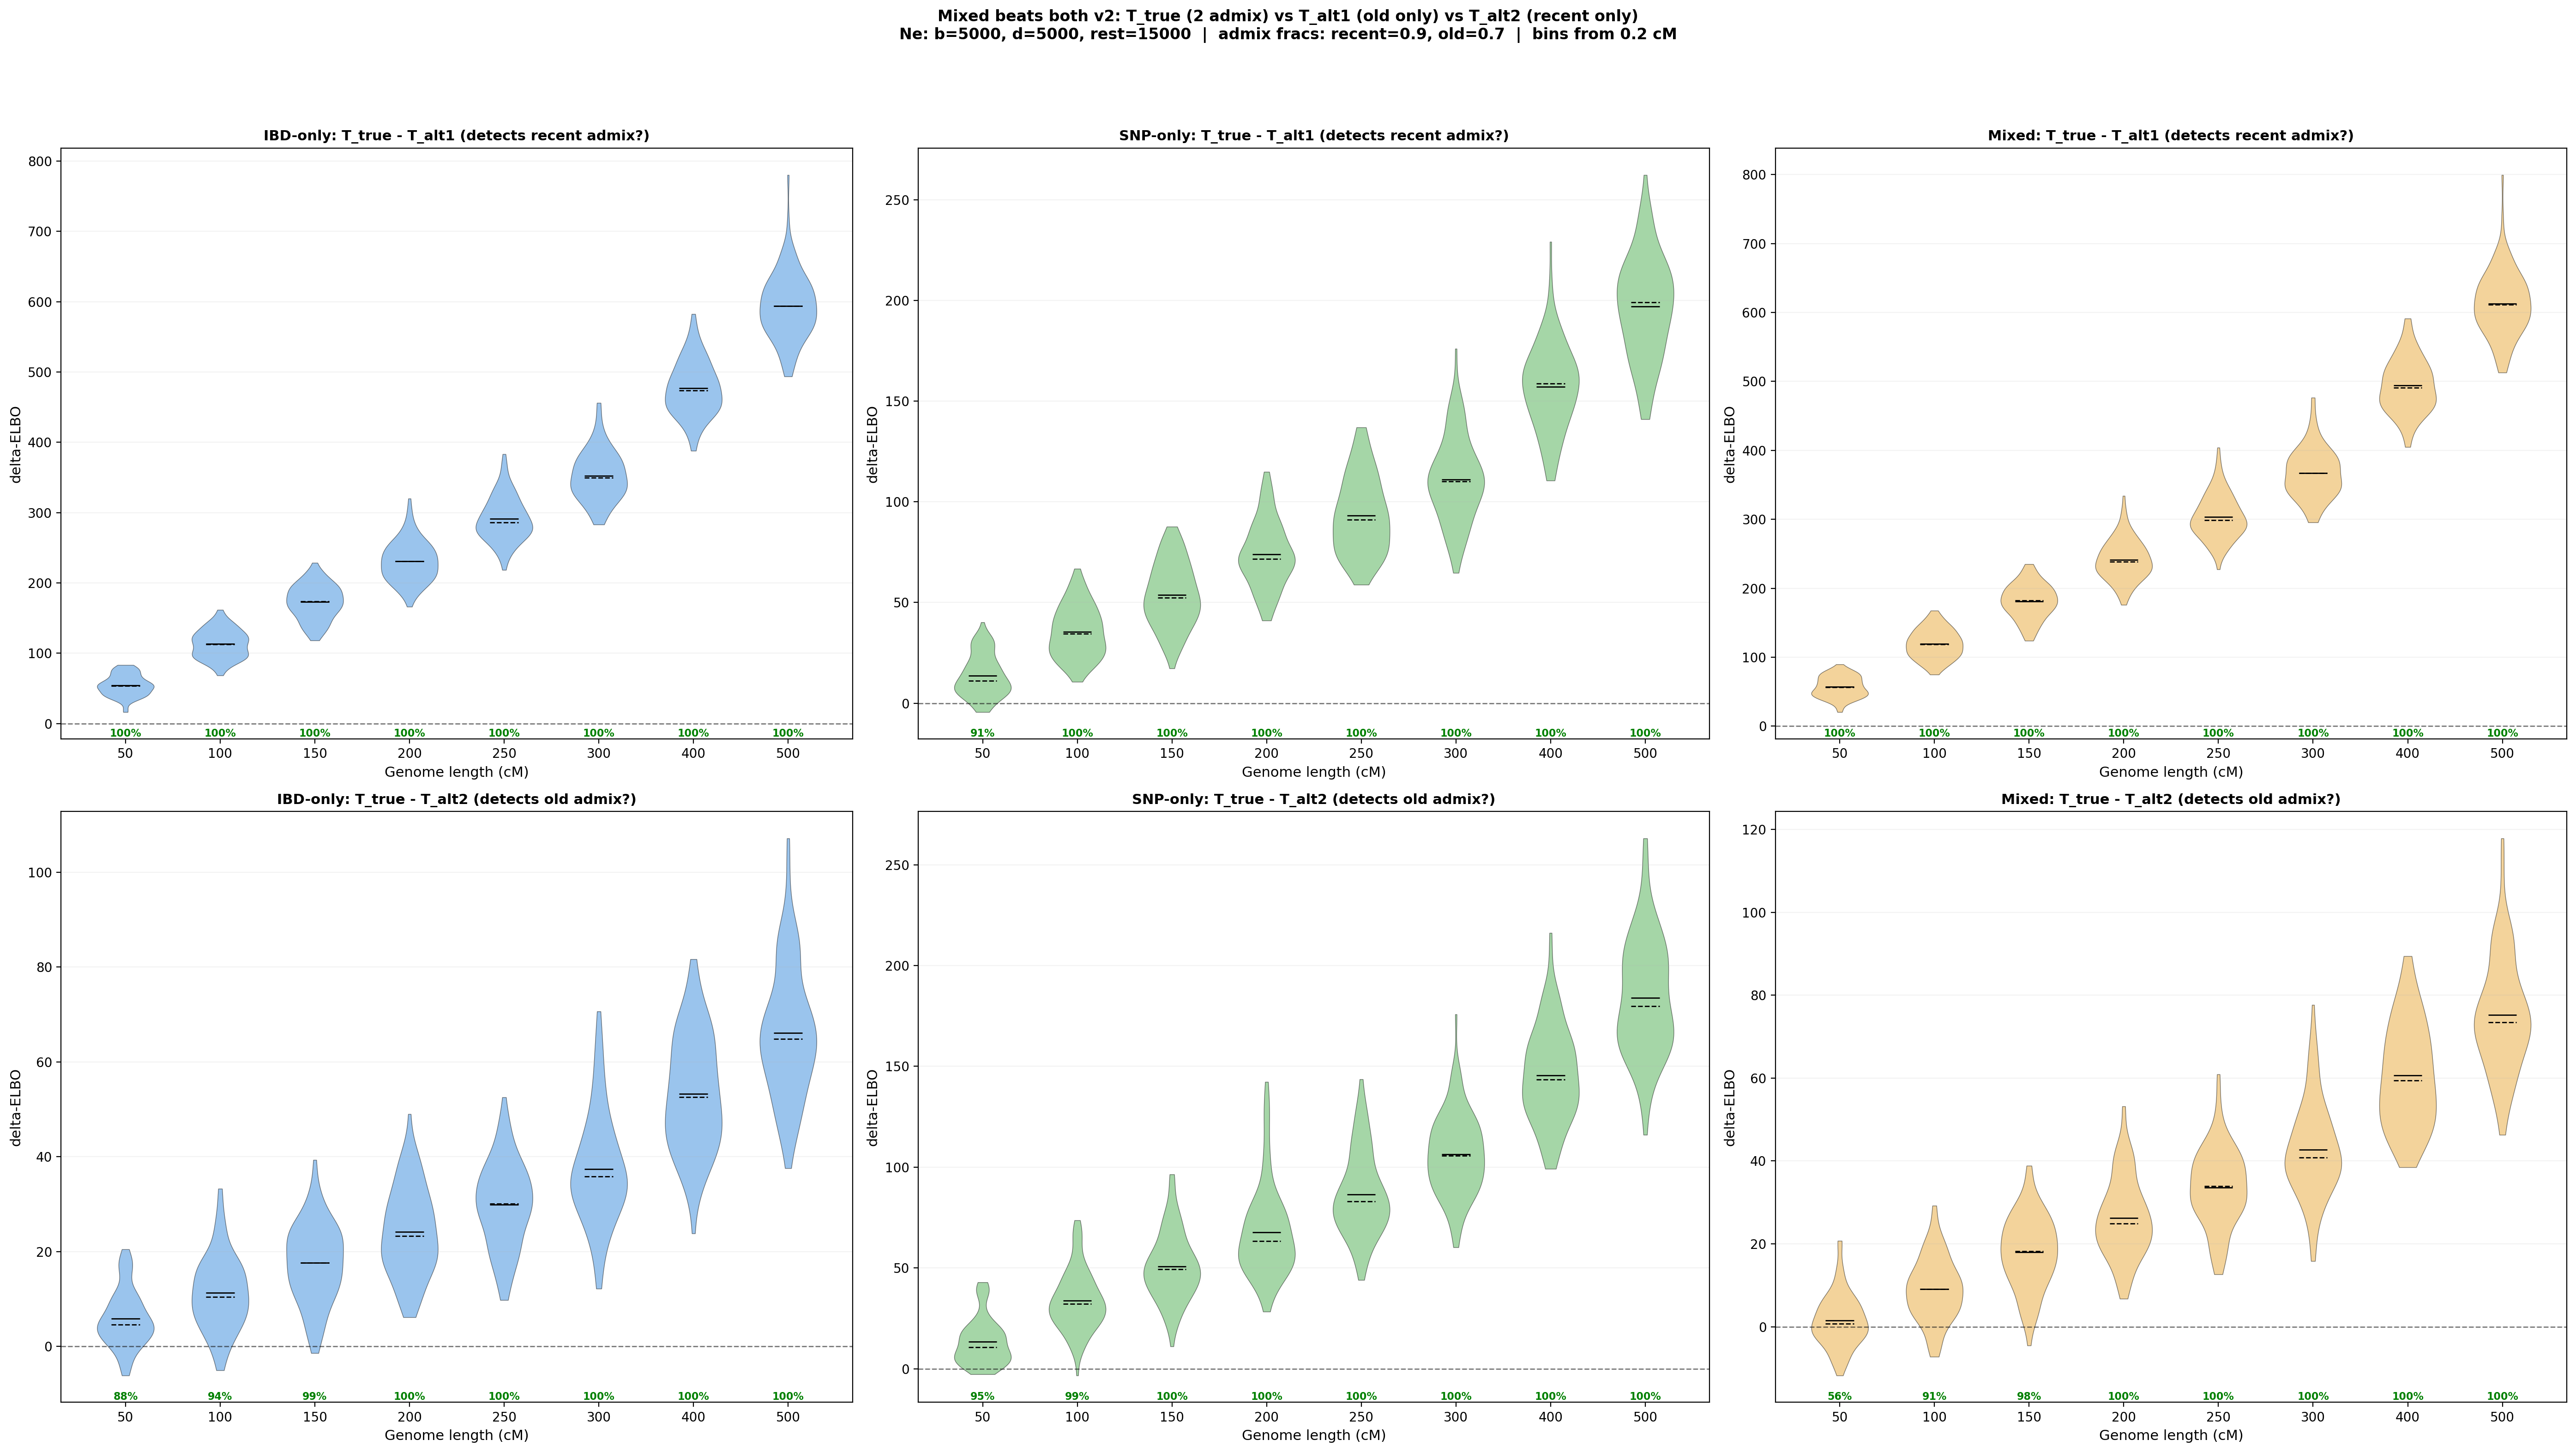
\includegraphics[width=\textwidth]{mixed_v2_dELBO.png}
        \caption{$\Delta\text{ELBO}$ for the varying-$N$ success case. Top row:
        $\text{true}-\text{alt1}$ (recent admixture). Bottom row:
        $\text{true}-\text{alt2}$ (old admixture). The Mixed model (orange) is
        positive earliest on both axes.}\label{fig:dELBO_v2}
    \end{figure}

\subsubsection{Failure: a pulse-count identifiability limit}
The second experiment is engineered to break the recent signal. Its true topology
(\cref{fig:topo_v4}) replaces the single recent admixture on $b$ with \emph{two}
pulses from the $a$-side (at $t=10$ and $t=80$) whose ancestry fractions sum to
the same net $50\%$, and keeps an old admixture on $d$. The competing
$\text{T}_{\text{alt1}}$ collapses the two pulses into a single recent pulse of
$50\%$ at an intermediate time. Because $f$-statistics depend only on \emph{net}
admixture proportions, not on the number of pulses (Maier \emph{et al.}, 2023),
the SNP covariance of the one-pulse and two-pulse models is essentially
identical; only the IBD segment-length distribution encodes the pulse timing (a
single $50\%$ pulse caps segment lengths around $1.2$ cM, leaving the $1.5$--$8$
cM bins as a structural-zero region that only the two-pulse history can
populate). \cref{fig:dELBO_v4} shows the limit: on the pulse-structure axis (top
row, $\text{true}-\text{alt1}$) every model --- including Mixed --- has
$\Delta\text{ELBO}$ centred \emph{below} zero, i.e. the data prefer the simpler
one-pulse explanation; the segment-length signal that should distinguish them is
too weak at these sizes and sample numbers to overcome the penalty for the extra
pulse. The old-admixture axis (bottom row, $\text{true}-\text{alt2}$) is still
recovered (IBD and Mixed positive), confirming the failure is specific to
pulse-count resolution and not a general breakdown. This case marks the current
boundary of what the composite likelihood can resolve and motivates the
finer-grained recent-length bins used in the \texttt{Nvarying} pipeline.

\begin{figure}[!htbp]
    \centering
        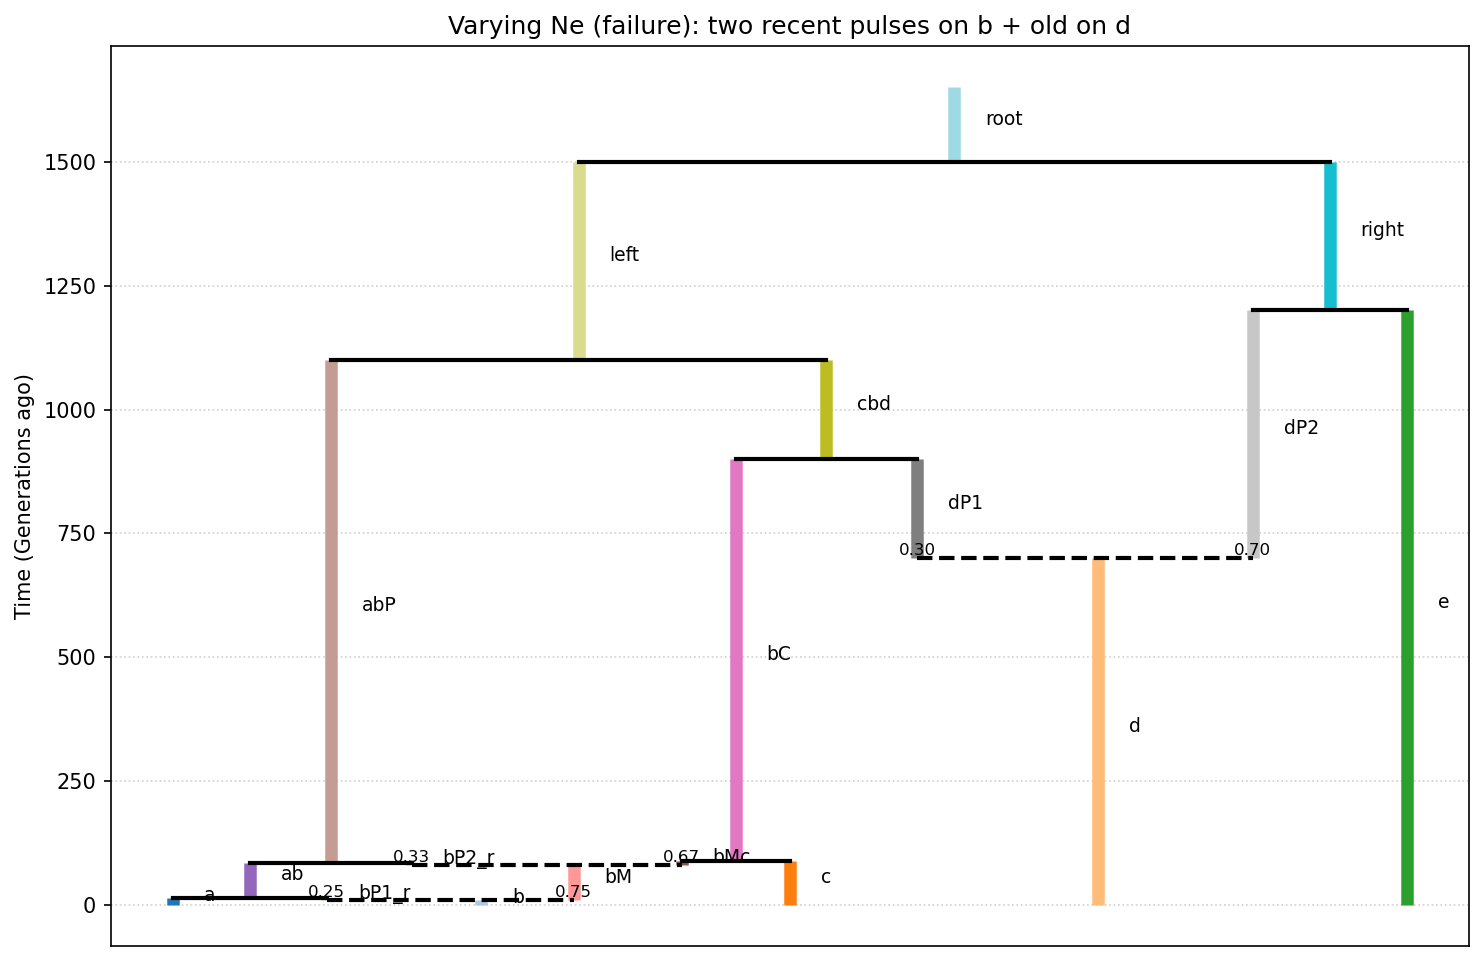
\includegraphics[width=13.5cm]{topology_mixed_v4.png}
        \caption{Varying-$N$ failure case (true topology): \emph{two} recent
        $a$-side pulses on $b$ ($t=10$ and $t=80$, net $50\%$) plus an old
        admixture on $d$ ($t=700$, $30\%$). The competitor merges the two pulses
        into one, which $f$-statistics cannot distinguish.}\label{fig:topo_v4}
    \end{figure}

\begin{figure}[!htbp]
    \centering
        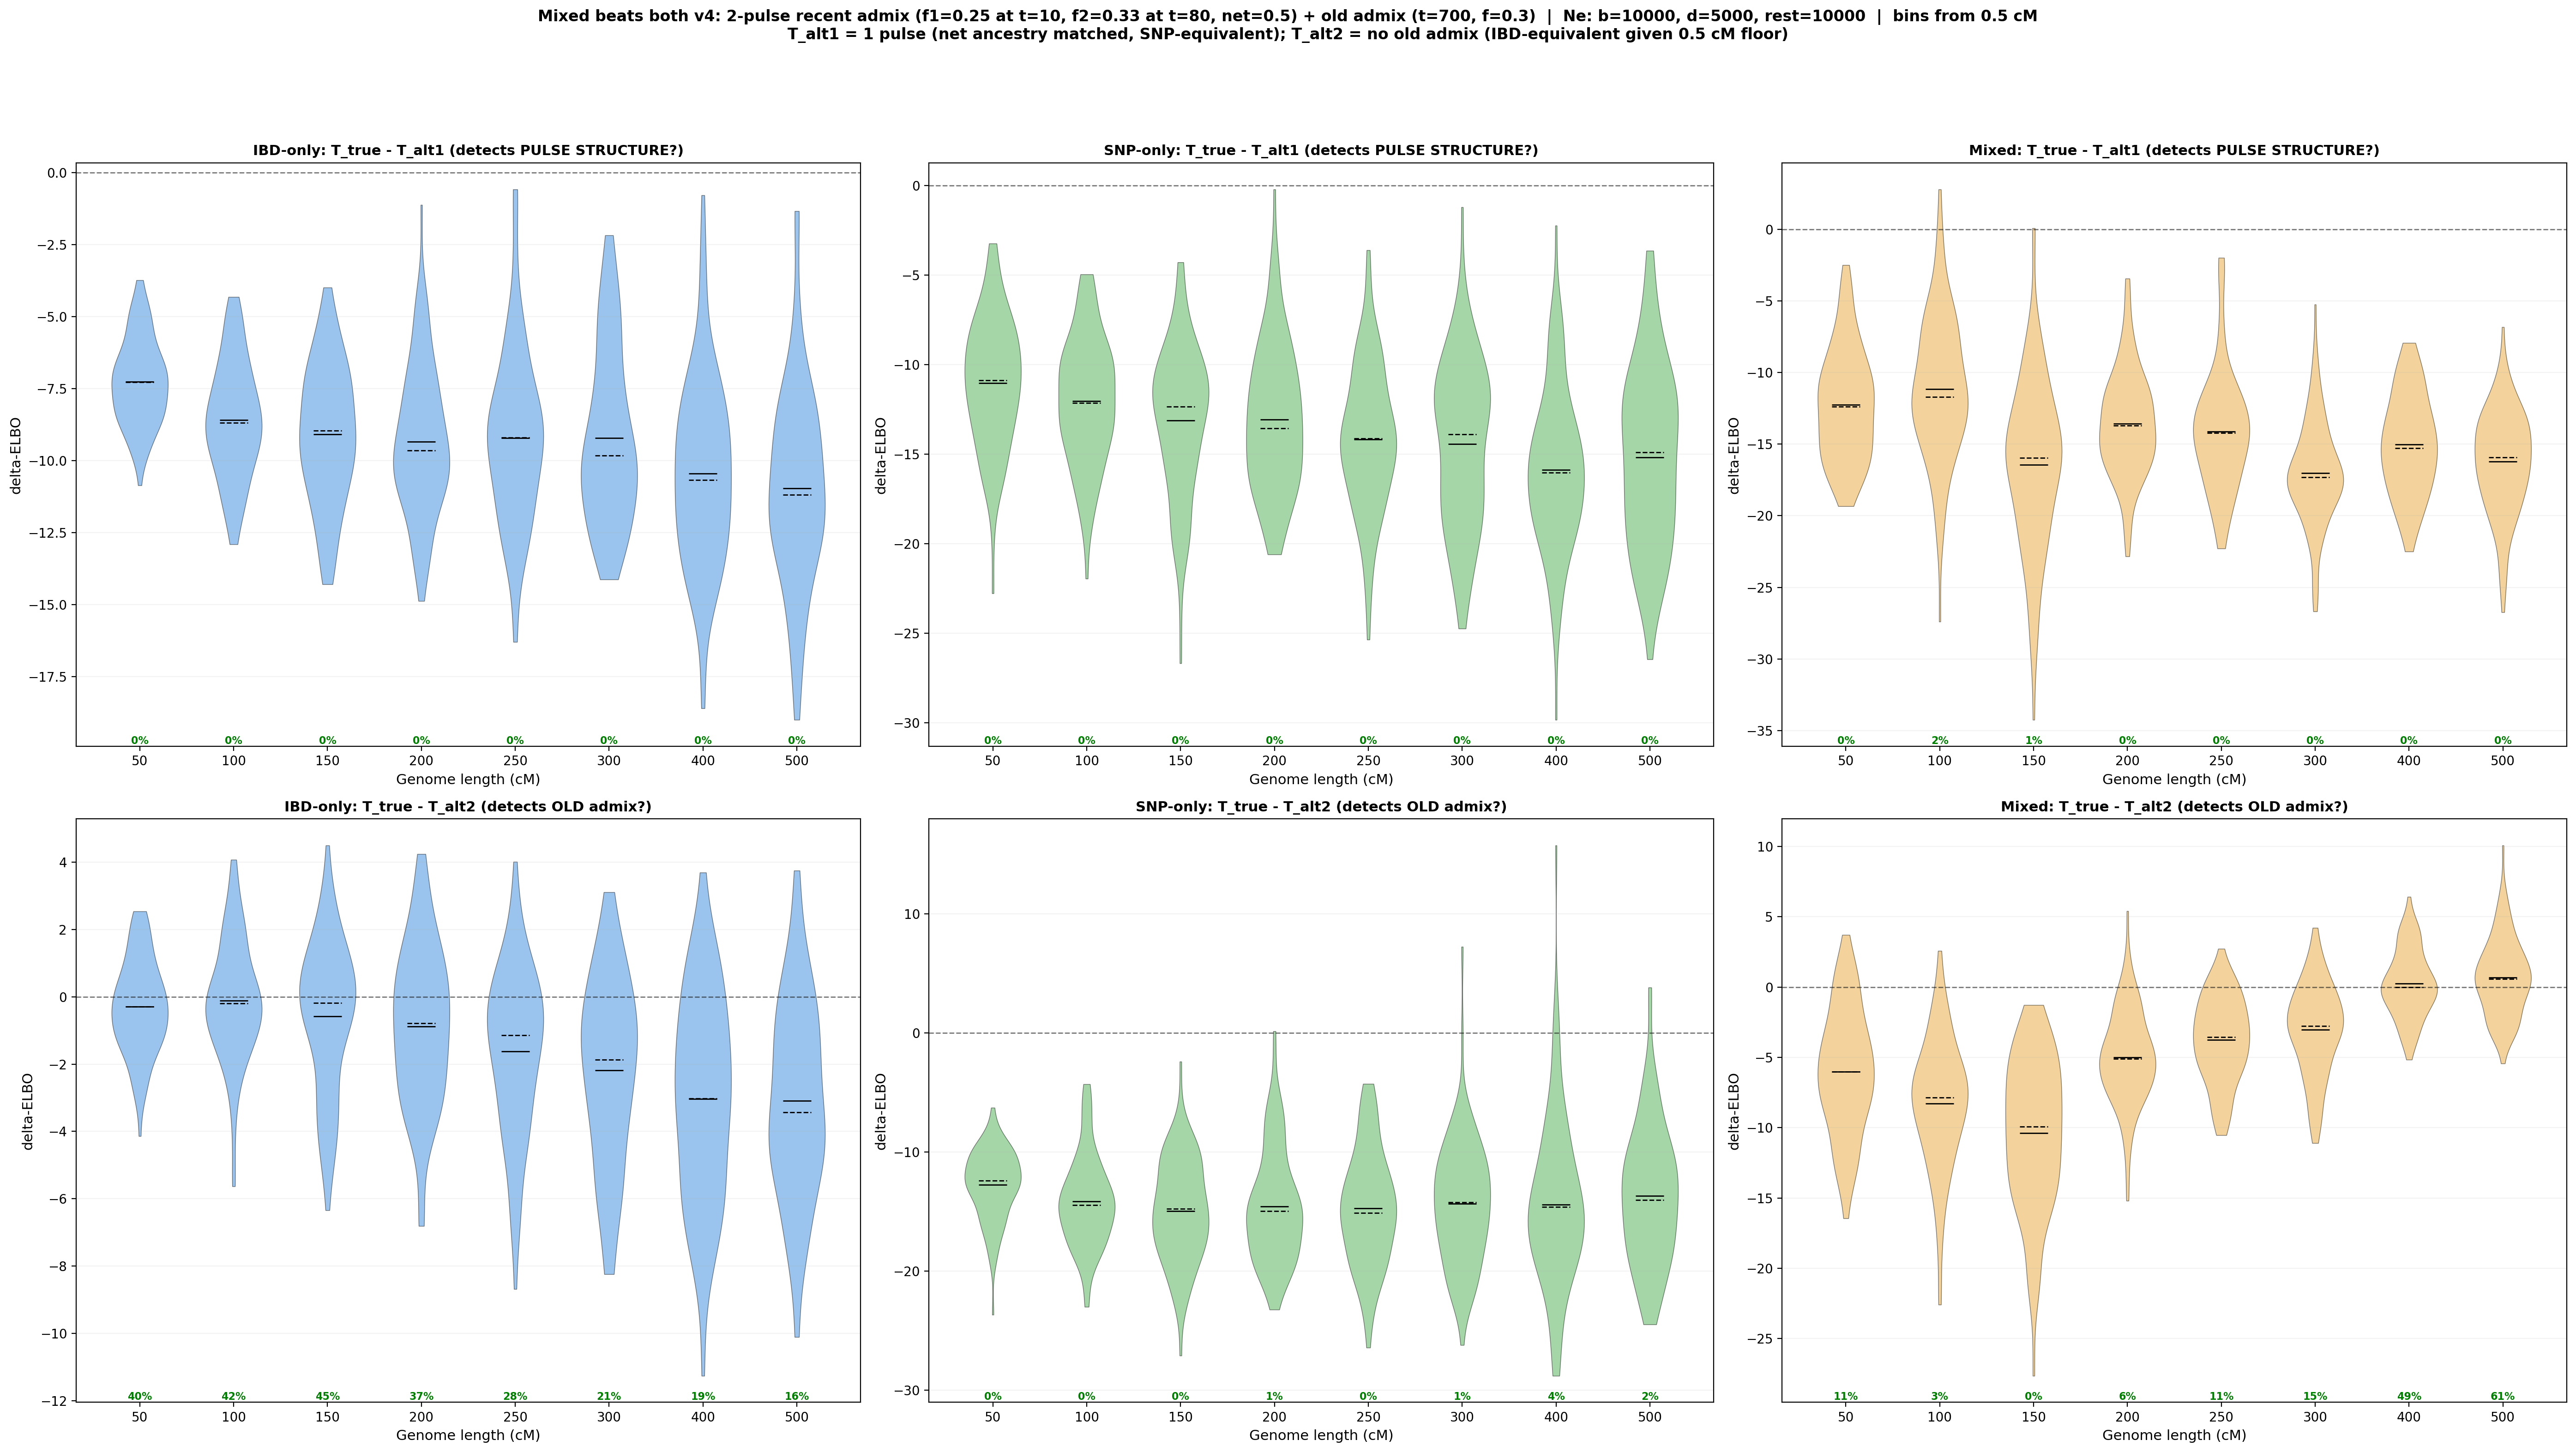
\includegraphics[width=\textwidth]{mixed_v4_dELBO.png}
        \caption{$\Delta\text{ELBO}$ for the varying-$N$ failure case. Top row
        (pulse-structure test, $\text{true}-\text{alt1}$): all models, including
        Mixed, sit below zero --- the two-pulse history is not resolved. Bottom
        row (old-admixture test): still recovered.}\label{fig:dELBO_v4}
    \end{figure}

Together the two cases show that the recent-versus-ancient division of labor
between IBD and SNP data carries over to the varying-$N$ regime --- the Mixed
model dominates when the events are individually resolvable --- while also
delimiting it: when two histories are deliberately constructed to share both
their $f$-statistics and (nearly) their IBD length spectrum, no amount of
combining the two modalities recovers the distinction.
\end{document}
